% !Mode:: "TeX:UTF-8"

\chapter[基于特征聚合与选择性扫描的无监督域迁移]{基于特征聚合与选择性扫描的无监督域迁移}[]
\chaptermark{基于特征聚合与选择性扫描的无监督域迁移}

% 图表与公式编号按章重置并显示为 "章-序"（X-Y）格式，
% 由 book.cls 的 \newcounter{figure}[chapter] / \@addtoreset{equation}{chapter}
% 与 hithesisbook.cls 的 \thefigure / \thetable 定义共同保证；
% 此处不可再调用 \counterwithin，它会把编号改写为 "X.Y" 且全局泄漏到后续章节。

\section{引言}

跨数据域分布偏移是模型迁移学习面临的核心挑战之一。由于源域与目标域在成像条件、视觉风格、背景结构和样本统计特性等方面存在差异，模型在源域中学习到的判别规则往往难以直接适用于目标域。当目标侧缺乏可靠监督信号时，模型只能依赖自身预测或结构先验完成适应，迁移误差便容易在训练过程中持续累积。如何在分布变化和监督缺失的双重约束下获得可靠的目标域模型，是跨域迁移研究需要解决的关键问题。
在数据隐私、存储成本和商业机密等现实约束下，源域样本通常无法在目标域适应阶段持续访问。与可同时使用源域和目标域数据的传统域适应方法相比，无源域适应（Source-Free Domain Adaptation, SFDA）仅保留预训练源模型，在不访问源域样本的条件下将其迁移至无标签目标域。此时，源样本重构、显式源—目标分布对齐和域判别等常用机制均难以直接采用，模型需要完全依赖目标域数据及源模型所携带的知识完成适应，因而进一步放大了迁移过程中的不确定性。

这种不确定性主要体现为两个相互耦合的层面。其一，骨干网络提取的表征能否在跨域后保持稳定的判别结构，决定了目标样本在特征空间中的可分性；其二，伪标签能否提供可靠监督，决定了自训练过程是否会朝正确方向更新。表征质量不足会降低伪标签可靠性，而错误伪标签又会通过迭代优化持续损害特征表征，形成表征退化与监督噪声相互强化的闭环。因此，可靠的无源域适应不仅需要抑制伪标签噪声，也需要增强跨域表征的鲁棒性。

作为跨域迁移伪标签自训练的主流技术路线之一，源假设迁移（Source-Hypothesis Transfer, SHOT）~\cite{liang2021source}提出的伪标签自训练框架已被广泛采纳并衍生出大量改进工作~\cite{fan2021dda,wang2025osda}，其基本流程可概括为三步：冻结源域分类器，以源模型对目标样本的初始预测为锚点进行聚类生成伪标签；以伪标签为监督信号并叠加信息最大化（Information Maximization, IM）~\cite{gomes2010discriminative}损失对特征提取器进行更新；通过迭代聚类—更新循环逐步精炼伪标签质量。然而，该框架的效果仍受限于特征表征和伪标签监督之间的耦合关系：当骨干网络缺乏对跨域稳定语义的有效建模时，聚类结果易受域特异性因素干扰；当伪标签包含噪声时，自训练又会放大错误监督，进而限制模型性能。

针对上述问题，本章将源—目标域差异引发的表征退化、伪标签噪声统一视为迁移不确定性的不同表现，并按不确定性的归属层次组织研究工作。
判别层的不确定性表现为伪标签噪声：只要基于聚类生成的伪标签发生错误分配，噪声就会通过自训练回路在判别层累积传播。
% 并沿卷积神经网络CNN与状态空间模型（State-Space Model, SSM）两条骨干路径开展研究。面向CNN 骨干，
针对该层次，本章提出基于特征聚合的不确定性感知伪标签去噪方法（Uncertainty-aware Pseudo-label-filtering Adaptation, UPA），借助特征空间邻居一致性估计样本级不确定性以自适应筛选高质量伪标签，并通过类感知对比学习阻断残余噪声的记忆传播，从去噪与对比正则两个角度抑制跨域迁移过程中判别层的不确定性传播。
表征层不确定性则与骨干的建模方式直接相关：状态空间模型以选择性扫描展开空间序列，其跨通道频率域依赖建模不足，且隐藏状态演化会记忆源域中前景与背景的空间共现模式。为此，本章在判别层去噪机制的基础上进一步提出基于选择性扫描的不确定性感知迁移方法（SfMamba），针对上述两类骨干相关的不确定性，通过通道级视觉状态空间模块显式建模跨通道频率域依赖以稳定源域表征，通过语义一致性打乱策略在自训练阶段主动扰乱背景 patch 的空间共现以阻断序列层虚假相关性的累积，以线性复杂度实现高效长程跨域建模。SfMamba 在状态空间骨干上沿用 UPA 的邻居感知去噪机制，使判别层去噪与骨干级增强在同一自训练框架中协同发挥作用。

本章在 Office、Office-Home、VisDA-C 和 DomainNet-126 四个 SFDA 基准上开展实验，验证所提方法在不同跨域任务中的有效性，并分析其在适应精度与计算效率之间的权衡。

本章工作可归纳为以下三点：
\begin{enumerate}
    \item 判别层不确定性抑制：提出基于特征空间邻居一致性的样本级不确定性估计方法与类感知对比学习策略，从去噪与对比正则两个角度协同抑制噪声标签的记忆传播。
    \item 表征层不确定性抑制：针对状态空间骨干在跨域迁移中特有的通道建模缺失与空间序列虚假相关性累积问题，分别设计通道级视觉状态空间模块与语义一致性打乱策略，在通用去噪组件之上形成骨干级增强。
    \item 在四个基准数据集上验证上述不确定性分层抑制机制的有效性，优于其他基线方法。
\end{enumerate}

\section{基于特征聚合的不确定性感知伪标签去噪方法}

\label{sec:chap2_upa}

本章两条方法均建立在统一的 SFDA 任务设定之上：给定带标签源域数据 $\mathcal{S} = \{(x_i^s, y_i^s)\}_{i=1}^{n_s}$ 与无标签目标域数据 $\mathcal{T} = \{x_i^t\}_{i=1}^{n_t}$，两者共享标签空间 $\mathcal{Y}$，且 $|\mathcal{Y}| = C$。源域与目标域的边缘分布存在差异，即 $Q(x) \neq P(x)$，但条件分布保持一致：$Q(y \mid x) = P(y \mid x)$。源域模型 $\theta_s = f \circ g$ 在源域数据 $\mathcal{S}$ 上完成预训练，其中 $g: \mathcal{X} \to \mathbb{R}^D$ 为特征提取器，$f: \mathbb{R}^D \to \mathbb{R}^C$ 为分类器。目标域适应阶段，源域数据 $\mathcal{S}$ 不可访问；目标模型 $\theta_t$ 以 $\theta_s$ 为初始化，仅通过目标域无标签数据进行自训练。本章两条方法均遵循以下基本设定：分类器 $f$ 在适应阶段保持冻结以提供稳定的任务锚点，仅对特征提取器 $g$ 进行更新，避免源域知识的灾难性遗忘。

两类方法均建立在 SHOT~\cite{liang2021source} 提出的伪标签自训练框架之上：首先利用源域模型的初始预测对目标域样本进行聚类，生成伪标签；随后采用信息最大化（IM）损失~\cite{gomes2010discriminative} 和伪标签监督损失对 $g$ 进行更新。SHOT 的局限在于：其通过伪标签噪声传播的累积误差对骨干架构的选择较为敏感，且CNN 骨干的局部感受野不足以捕获跨域不变的长程特征依赖。本章的 UPA 与 SfMamba 分别从判别层去噪与表征—序列双层增强两个角度改进该框架，统一体现为对迁移不确定性的抑制。具体地，设当前模型对目标样本 $x^t$ 的预测概率分布为 $p(x^t) = \delta(\theta_t(x^t))$（$\delta$为Softmax函数），按 SHOT 范式进行迭代聚类：
\begin{equation}
\boldsymbol{\mu}^{(k)}_c = \frac{\sum_{x^t \in \mathcal{T}} \mathbf{1}(\hat{y}^{(k)}_t = c) \, g(x^t)}{\sum_{x^t \in \mathcal{T}} \mathbf{1}(\hat{y}^{(k)}_t = c)}, \qquad
\hat{y}^{(k+1)}_t = \arg\max_c \, d\!\left(g(x^t), \boldsymbol{\mu}^{(k)}_c\right),
\label{eq:chap2_proto}
\end{equation}
其中 $d(\cdot, \cdot)$ 为余弦相似度，$\mathbf{1}(\cdot)$ 为指示函数。经验上两轮迭代即可收敛，记最终伪标签为 $\hat{y}_t$。借鉴 IM 损失，对模型预测熵最小化来鼓励对单样本给出确定性预测，并且使用多样性正则化来防止预测集中于少数类别：
\begin{equation}
\mathcal{L}_{\text{IM}} = \mathcal{L}_{\text{ent}} + \mathcal{L}_{\text{div}}, \quad
\mathcal{L}_{\text{ent}} = -\mathbb{E}_{x^t} \sum_c p_c(x^t) \log p_c(x^t), \quad
\mathcal{L}_{\text{div}} = \sum_c \hat{p}_c \log \hat{p}_c,
\label{eq:chap2_im}
\end{equation}
其中 $\hat{p} = \mathbb{E}_{x^t}[p(x^t)]$ 为平均预测分布。$\mathcal{L}_{\text{div}}$ 通过惩罚 $\hat{p}$ 偏离均匀分布 $1/C$ 来促进类别平衡。

判别层是伪标签自训练范式中迁移不确定性的主要载体。骨干结构会影响这一噪声的严重程度。以 CNN 为例，其特征空间虽具备层次化聚合能力，但固定局部感受野对跨域长程依赖建模不足，使得基于聚类得到的伪标签不可避免地包含错误分配，而噪声的载体始终是判别层的伪标签本身。
这些错误标签通过自训练回路在判别层累积传播，构成 CNN 骨干路径上迁移不确定性的核心来源。UPA 的核心动机来自一个关键实验观察：在 VisDA-C 数据集上，若人工剔除 SHOT 生成的错误伪标签（SHOT-clean），适应精度从 82.9\% 显著提升至 88.4\%（图~\ref{fig:motivation_shot}），揭示自训练范式的性能上限很大程度上被判别层伪标签噪声所限制。现有判别层去噪方法依赖额外的辅助模型，例如双分类器~\cite{liang2021source}、动量平均模型~\cite{tarvainen2017mean} 等，来估计不确定性，但额外模型的预测偏差会引入新的建模误差。UPA 的关键观察是：在 CNN 特征空间中，正确伪标签对应的样本聚集紧密形成清晰类别簇，而错误伪标签对应的样本散布于类别边界或簇间区域（图~\ref{fig:feat_cluster}），这一聚类结构差异使得邻居分布成为无需额外模型的样本级不确定性估计来源。基于此，UPA 提出了由粗到精的二阶段去噪流水线，如图~\ref{fig:framework}所示：第一阶段通过自适应伪标签选择模块基于特征空间邻居一致性将目标域样本划分为干净集 $\mathcal{T}_c$ 与噪声集；第二阶段通过类感知对比学习策略在干净集上实施类别级对比学习，阻断残余噪声在表征空间的记忆传播。两阶段共同实现对判别层迁移不确定性的由粗到精抑制。

\begin{figure}[!htbp]
    \centering
    \setlength{\tabcolsep}{0pt}
    \subfigure[]{%
      \includegraphics[width=0.48\linewidth]{papers/UPA/fig_1_v3.pdf}
      \label{fig:motivation_shot}%
    }\hfill
    \subfigure[]{%
      \includegraphics[width=0.48\linewidth]{papers/UPA/re-fig1_2.pdf}
      \label{fig:feat_cluster}%
    }
    \bicaption[fig:upa_motivation]{}{UPA 的两个动机观察}{Fig.}{Two motivation observations of UPA}
\end{figure}

\begin{figure*}[!htbp]
  \centering
  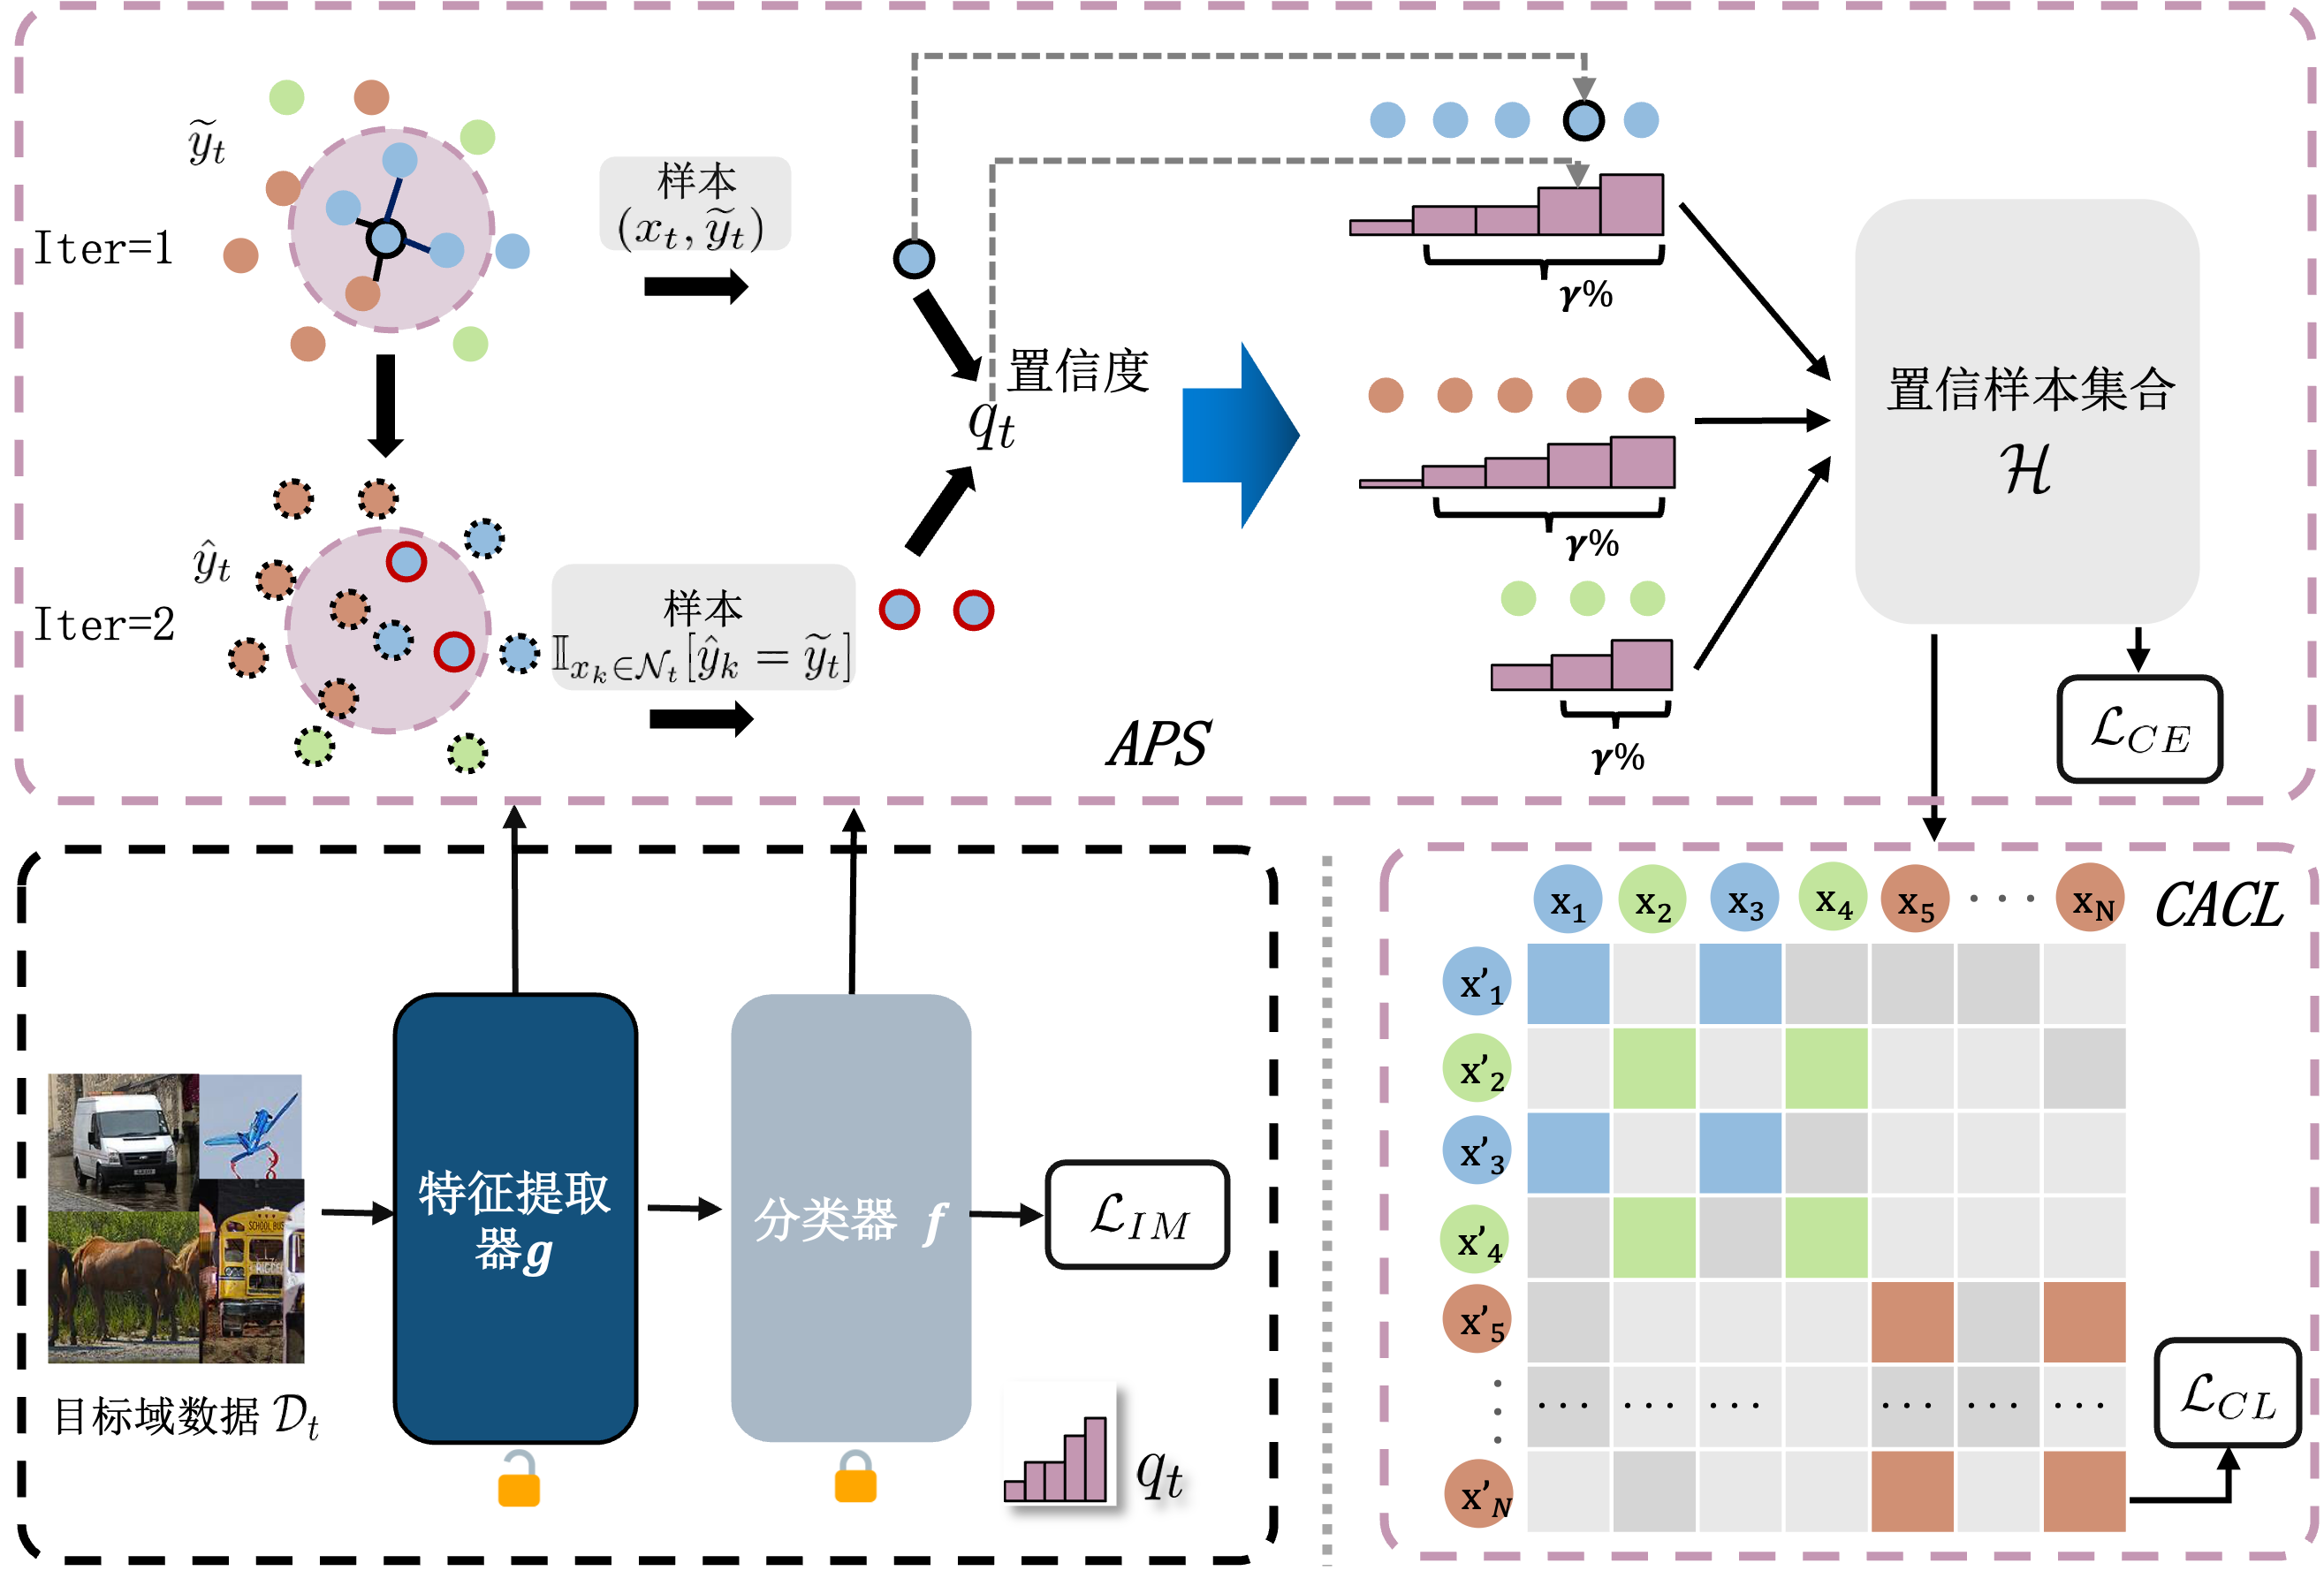
\includegraphics[width=0.85\textwidth]{figures/upa_extracted/v6_framework.png}
  \bicaption[fig:framework]{}{UPA 方法整体框架}{Fig.}{Overall framework of UPA.}
\end{figure*}

\subsection{邻域一致性驱动的判别层去噪}

\label{sec:chap2_upa_denoising}

我们假设：在特征空间 $g(x_t)$ 中，那些易于聚类的样本因同一类别内存在相似特征而包含更高程度的域共享信息；相比之下，大量不确定样本则分布在聚类中心之间，这主要源于域间的分布偏移。受此启发，我们提出了一种新颖的伪标签去噪机制（Adaptive Pseudo-label Selection, APS），该机制通过近邻样本来迭代评估样本的不确定性：

对所有目标样本的特征向量 $\ell_2$ 归一化后，计算两两余弦相似度构成相似度矩阵 $\mathbf{S}_t \in \mathbb{R}^{n_t \times n_t}$。对每个样本 $x_t$，取相似度最高的 $K$ 个样本（不含自身）作为其 K 近邻集合 $\mathcal{N}_t$。

APS 通过邻居集合进行距离加权投票，估计样本 $x_t$ 的类别后验概率 $\hat{p}_t \in \mathbb{R}^C$：

\begin{equation}
\hat{p}_t = \frac{1}{K} \sum_{x_k \in \mathcal{N}_t} d\!\left(g(x_t), g(x_k)\right) e_{\hat{y}_k},
\label{eq:knn_voting}
\end{equation}
其中 $e_{\hat{y}_k} \in \mathbb{R}^C$ 为伪标签 $\hat{y}_k$ 的 one-hot 向量。临时伪标签通过下式更新：
\begin{equation}
\hat{y}_t = \arg\max_c \, \hat{p}_t^{(c)}.
\label{eq:label_update}
\end{equation}

实验验证，两轮迭代即可收敛。该估计过程完全发生在特征空间内部，无需任何额外模型，符合特征空间自洽性的核心命题。
在不确定性估计完成后，本文用置信度评分 $q_t$ 来量化伪标签质量：
\begin{equation}
q_t = \frac{1}{K} \sum_{x_k \in \mathcal{N}_t} \mathbf{1}\!\left(\hat{y}_k = \hat{y}_t\right) d\!\left(g(x_t), g(x_k)\right).
\label{eq:confidence}
\end{equation}
$q_t$如图~\ref{fig:confidence_score}所示实际衡量了样本的邻域一致性，仅与最终伪标签 $\hat{y}_t$ 一致的邻居通过余弦相似度 $s$ 贡献于 $q_t$，
邻域预测越一致伪标签越可靠。

\begin{figure}[!htbp]
  \centering
  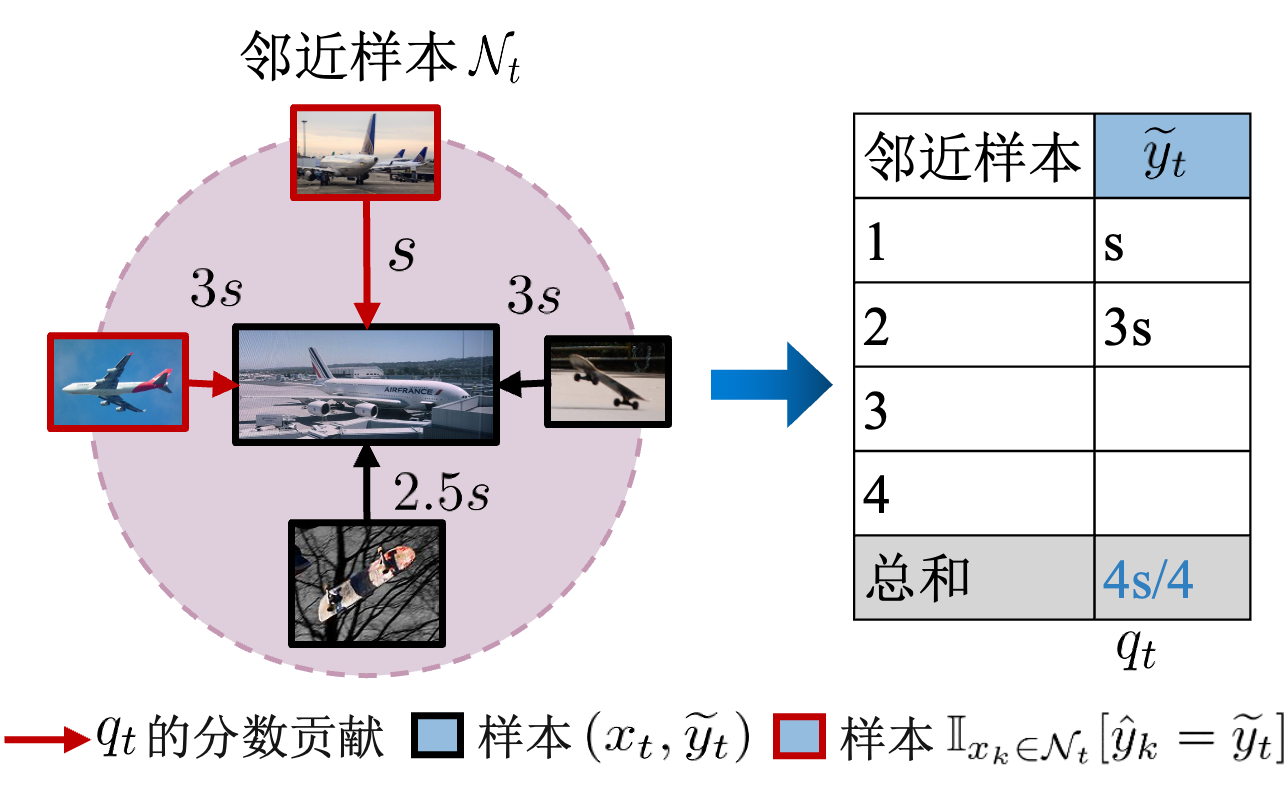
\includegraphics[width=0.55\textwidth]{figures/upa_extracted/v6_Aps.png}
  \bicaption[fig:confidence_score]{}{置信度评分 $q_t$ 的几何解释}{Fig.}{Geometric interpretation of confidence score $q_t$}
\end{figure}

此外，为避免在筛选过程中遗漏少数类，按 $q_t$ 对各类别内的样本分别排序，选取每个类别中得分最高的前 $\gamma_{\text{sel}}\%$ 的样本，组成干净伪标签样本集 $\mathcal{T}_c$。类别内排序策略在保证各类别均有样本入选的同时，使筛选阈值由类别内的置信度分布自适应决定。

\subsection{类感知对比学习策略}

\label{sec:chap2_upa_cacl}

尽管 APS 能够过滤大部分噪声伪标签，但仍不可避免地存在少量漏网的错误伪标签，以及类别边界区域的歧义样本。这些残余噪声会通过自训练回路在表征空间中被模型记忆，构成迁移不确定性的隐蔽来源。为此，本文提出类感知对比学习（Class-Aware Contrastive Learning, CACL）策略，在干净伪标签样本集 $\mathcal{T}_c$ 上利用类别级对比学习增强类内语义一致性，阻断噪声记忆的传播。

对于每个样本 $x_i$，首先生成其强增强视图 $x_i'$，在大小为 $B_{\text{batch}}$ 的 mini-batch 中，我们定义$i\in \mathcal{I}=\{1,\cdots,2B_{\text{batch}}\}$, 若两个样本 $(x_i, y_i)$ 和 $(x_j, y_j)$ 均属于 $\mathcal{T}_c$ 且 $y_i = y_j$，则二者构成正样本对：
\begin{equation}
\mathcal{O}(i) = \left\{ o_{ij} \mid y_i = y_j;\ (x_i, y_i), (x_j, y_j) \in \mathcal{T}_c \right\},
\label{eq:positive_pairs}
\end{equation}
其中 $o_{ij} = \langle (x_i, y_i), (x_j, y_j) \rangle$，$j \in \mathcal{A}(i) \equiv \mathcal{I} \setminus \{i\}$。类别级对比损失形式化为：
\begin{equation}
\mathcal{L}_{\text{CL}} = \sum_{i \in \mathcal{I}} -\frac{1}{|\mathcal{J}(i)|} \sum_{j \in \mathcal{J}(i)} \log \frac{\exp(z_i \cdot z_j / \tau)}{\sum_{a \in \mathcal{A}(i)} \exp(z_i \cdot z_a / \tau)},
\label{eq:contrastive_loss}
\end{equation}
其中 $\mathcal{J}(i) = \{j \mid j \in \mathcal{A}(i), o_{ij} \in \mathcal{O}(i)\}$，$\tau$ 为温度参数，$z_i = g(x_i)/\|g(x_i)\|$ 为归一化特征。CACL 通过强增强视图间的类内一致性约束，增强目标域上的判别性表征，并有效阻断模型对残余噪声伪标签的记忆。

除 CACL 外，UPA 采用标准交叉熵损失引导模型在干净伪标签样本集上的学习：
\begin{equation}
\mathcal{L}_{\text{CE}} = -\mathbb{E}_{(x_t, \hat{y}_t) \in \mathcal{T}_c} \sum_{c=1}^{C} \mathbf{1}(c = \hat{y}_t) \log p_c(x_t),
\label{eq:ce_loss}
\end{equation}

最终总体损失为 $\mathcal{L} = \mathcal{L}_{\text{CL}} + \beta_{\text{CE}} \mathcal{L}_{\text{CE}} + \mathcal{L}_{\text{IM}}$。完整训练流程以渐进式适应方式交替执行 APS 伪标签筛选与基于总体损失的参数更新，如算法~\ref{alg:upa} 所示。

\begin{algorithm}[!htb]
  \AlgoBiCaption{UPA 算法训练流程}{Training procedure of UPA}
  \label{alg:upa} 
  \small
  \KwIn{无标签目标样本 $\mathcal{T}$，预训练源域模型 $\theta_s$；训练轮数 $\hat{T}$，每轮迭代数 $e_T$，批次大小 $B_{\text{batch}}$；超参数 $\gamma_{\text{sel}}, \tau, K, \beta_{\text{CE}}$}
  \KwOut{适应后的目标域模型 $\theta_t$}
  \BlankLine
  \For{epoch $= 1$ \textbf{to} $\hat{T}$}{
    基于式\eqref{eq:chap2_proto} 生成伪标签 $\hat{y}_t$\;
    % \tcp{// APS 模块}
    基于式\eqref{eq:knn_voting}--\eqref{eq:confidence} 计算置信度评分并选取 top $\gamma_{\text{sel}}\%$ 样本构成 $\mathcal{T}_c$\;
    \For{iter $= 1$ \textbf{to} $e_T$}{
      从 $\mathcal{T}$ 中采样小批量样本 $\{x_b\}_{b=1}^{B_{\text{batch}}}$\;
      基于式\eqref{eq:positive_pairs} 构建正样本对集合 $\mathcal{O}$\;
      $\theta_t \leftarrow \theta_t - \eta \nabla (\mathcal{L}_{\text{CL}} + \beta_{\text{CE}} \mathcal{L}_{\text{CE}} + \mathcal{L}_{\text{IM}})$;
    }
  }
  \Return $\theta_t$
\end{algorithm}

\subsection{实验结果与分析}

\noindent\textbf{(1) 数据集与实验设置}

本节在 Office~\cite{saenko2010adapting}、Office-Home~\cite{venkateswara2017deep}、VisDA-C~\cite{peng2017visda} 与 DomainNet-126~\cite{peng2019moment} 四个基准数据集上评估 UPA 方法。具体而言：Office 数据集包含 Amazon（A）、Dslr（D）与 Webcam（W）三个域，域间共享31个类别；Office-Home 数据集包含 Art（A）、Clipart（C）、Product（P）与 Real World（R）四个域，每个域共享 65 个类别；VisDA-C 数据集包含合成域 Synthetic（S）与真实域 Real（R）的跨域分割任务；DomainNet-126 包含126个类别，来自 Real（R）、Painting（P）、Clipart（C）与 Sketch（S）四个域。实验对比了有源域数据的传统 UDA 方法（CDAN~\cite{CDAN}、MCC~\cite{MCC}、MDD~\cite{MDD}、BCDM~\cite{BCDM}、FixBi~\cite{FIxBi}、CAN~\cite{CAN}、SRDC~\cite{SRDC}、RSDA~\cite{RSDA}）与当前主流的 SFDA 方法（3C-GAN~\cite{3C-GAN}、U-SFAN~\cite{U-SFAN}、DIPE~\cite{DIPE}、HCL~\cite{HCL}、NRC~\cite{yang2021neighbor}、CoWA-JMDS~\cite{cowa}、AdaContrast~\cite{AdaContrast}、CDCL~\cite{wang2022cross}、D-MCD~\cite{chu2022denoised}、VDM-DA~\cite{tian2022vdm}、SSNLL~\cite{chen2022self}、SHOT~\cite{liang2021source}、Tent~\cite{tent}）。所有方法均采用 ResNet 作为骨干网络，其中 Office、Office-Home 与 DomainNet-126 使用 ResNet-50，VisDA-C 使用 ResNet-101。实验遵循 SHOT 框架的设置：冻结分类器参数，仅微调特征提取器。

训练阶段采用 SGD 优化器，设置动量 0.9、权重衰减 $10^{-3}$、batch size 64，学习率策略为先线性预热一个 epoch 后余弦退火衰减。Office、Office-Home 与 DomainNet-126 的初始学习率设为 $10^{-2}$，VisDA-C 的初始学习率设为 $10^{-3}$。瓶颈层学习率设置为骨干网络的 10 倍。超参数设置为：损失权重 $\beta_{\text{CE}} = 0.3$，对比温度 $\tau = 0.1$，近邻数 $K = 4$，各类数据集的置信样本筛选比例 $\gamma_{\text{sel}}$ 在Office/Office-Home/DomainNet-126设为 0.6, 在VisDA-C设为 0.8。
% 对比学习中的数据增强策略遵循 MoCoV2~\cite{chen2020momentum} 的设置。

\noindent\textbf{(2) 主实验结果}

\begin{table*}[!htbp]
  \bicaption[table:Visda-C]{}{UPA 在 VisDA-C 数据集上的准确率对比}{Table}{Comparison of accuracy of UPA on VisDA-C dataset. ResNet-101 is used as backbone and 'SF' means source-free. S$\to$R means Synthesis$\to$Real.}
  \vspace{0.5em}\centering\wuhao
  
  \resizebox{\textwidth}{!}{
  \begin{tabular}{lcccccccccccccc}
  \toprule
  Method (S$\to$R) & SF & plane & bcycl & bus & car & horse & knife & mcycl & person & plant & sktbrd & train & truck & Avg.\\
  \midrule
  CDAN~\cite{CDAN} & \ding{55} & 85.2 & 66.9 & 83.0 & 50.8 & 84.2 & 74.9 & 88.1 & 74.5 & 83.4 & 76.0 & 81.9 & 38.0 & 73.9\\
  MCC~\cite{MCC} & \ding{55} & 88.7 & 80.3 & 80.5 & 71.5 & 90.1 & 93.2 & 85.0 & 71.6 & 89.4 & 73.8 & 85.0 & 36.9 & 78.8\\
  BCDM~\cite{BCDM} & \ding{55} & 95.1 & 87.6 & 81.2 & 73.2 & 92.7 & 95.4 & 86.9 & 82.5 & 95.1 & 84.8 & 88.1 & 39.5 & 83.4\\
  FixBi~\cite{FIxBi} & \ding{55} & 96.1 & 87.8 & 90.5 & 90.3 & 96.8 & 95.3 & 92.8 & 88.7 & 97.2 & 94.2 & 90.9 & 25.7 & 87.2\\
  CAN~\cite{CAN} & \ding{55} & 97.0 & 87.2 & 82.5 & 74.3 & 97.8 & 96.2 & 90.8 & 80.7 & 96.6 & 96.3 & 87.5 & 59.9 & 87.2\\
  \midrule
  $-$ & $-$ & 56.9 & 22.6 & 49.5 & 75.8 & 62.5 & 6.7 & 83.3 & 27.2 & 58.3 & 42.0 & 82.0 & 6.4 & 47.8\\
  3C-GAN~\cite{3C-GAN} & \Checkmark & 94.8 & 73.4 & 68.8 & 74.8 & 93.1 & 95.4 & 88.6 & 84.7 & 89.1 & 84.7 & 83.5 & 48.1 & 81.6\\
  U-SFAN~\cite{U-SFAN} & \Checkmark & 94.9 & 87.4 & 78.0 & 56.4 & 93.8 & 95.1 & 80.5 & 79.9 & 90.1 & 90.1 & 85.3 & 60.4 & 82.7\\
  DIPE~\cite{DIPE} & \Checkmark & 95.2 & 87.6 & 78.8 & 55.9 & 93.9 & 95.0 & 84.1 & 81.7 & 92.1 & 88.9 & 85.4 & 58.0 & 83.1\\
  HCL~\cite{HCL} & \Checkmark & 93.3 & 85.4 & 80.7 & 68.5 & 91.0 & 88.1 & 86.0 & 78.6 & 86.6 & 88.8 & 80.0 & 74.7 & 83.5\\
  VDM-DA~\cite{tian2022vdm} & \Checkmark & 96.9 & 90.0 & 80.0 & 64.4 & \textbf{96.8} & 96.4 & 86.7 & 83.3 & 96.2 & 87.9 & 89.8 & 54.7 & 85.3\\
  NRC~\cite{yang2021neighbor} & \Checkmark & 96.8 & \textbf{91.3} & 82.4 & 62.4 & 96.2 & 95.9 & 86.1 & 80.6 & 94.8 & 94.1 & 90.4 & 59.7 & 85.9\\
  SSNLL~\cite{chen2022self} & \Checkmark & \textbf{98.3} & 88.2 & 88.1 & 79.7 & 96.5 & 90.4 & \textbf{92.5} & 81.6 & 92.9 & 86.3 & 91.9 & 45.4 & 86.0\\
  AdaContrast~\cite{AdaContrast} & \Checkmark & 97.0 & 84.7 & 84.0 & 77.3 & 96.7 & 93.8 & 91.9 & 84.8 & 94.3 & 93.1 & \textbf{94.1} & 49.7 & 86.8\\
  CoWA-JMDS~\cite{cowa} & \Checkmark & 96.2 & 89.7 & 83.9 & 73.8 & 96.4 & 97.4 & 89.3 & 86.8 & 94.6 & 92.1 & 88.7 & 53.8 & 86.9\\
  CDCL~\cite{wang2022cross} & \Checkmark & 97.3 & 90.5 & 83.2 & 59.9 & 96.4 & \textbf{98.4} & 91.5 & 85.6 & 96.0 & 95.8 & 92.0 & 63.8 & 87.5\\
  D-MCD~\cite{chu2022denoised} & \Checkmark & 97.0 & 88.0 & \textbf{90.0} & \textbf{81.5} & 95.6 & 98.0 & 86.2 & \textbf{88.7} & 94.6 & 92.7 & 83.7 & 53.1 & 87.5\\
  \midrule
  SHOT~\cite{liang2021source} & \Checkmark & 94.3 & 88.5 & 80.1 & 57.3 & 93.1 & 94.9 & 80.7 & 80.3 & 91.5 & 89.1 & 86.3 & 58.2 & 82.9\\
  \textbf{UPA} & \Checkmark & \textbf{97.0} & \textbf{90.4} & \textbf{82.6} & \textbf{65.0} & \textbf{96.7} & \textbf{96.7} & \textbf{91.0} & \textbf{87.0} & \textbf{96.8} & \textbf{96.5} & \textbf{89.2} & \textbf{75.0} & \textbf{88.7}\\
  \bottomrule
  \end{tabular}
  }
\end{table*}

如表~\ref{table:Visda-C}所示，UPA 在 VisDA-C 数据集上取得 88.7\% 的平均分类精度，显著超越 SHOT 基线方法，提升幅度达 5.8 个百分点。这一大幅提升充分验证了 APS 模块在过滤伪标签噪声方面的有效性。与此前最先进的 SFDA 方法 D-MCD相比，UPA 仍高出 1.2 个百分点，进一步确立了本方法在无源域适应任务中的优势。
值得注意的是，UPA 在多个细粒度类别上展现出尤为显著的提升。在卡车（truck）类别上，UPA 达到 75.0\% 的精度，相比 SHOT 的 58.2\% 提升了 16.8 个百分点；在汽车（car）类别上，UPA 达到 65.0\%，相比 SHOT 的 57.3\% 提升了 7.7 个百分点。这些类别具有明显的域间外观差异，说明 APS 模块通过 $K$ 近邻投票机制能够有效识别并剔除域偏移导致的噪声伪标签。

\begin{table*}[!htbp]
  \bicaption[table:office-home]{}{UPA 在 Office-Home 数据集上的准确率对比}{Table}{UPA classification accuracy on Office-Home. ResNet-50 is used as backbone and 'SF' means source-free.}
  \vspace{0.5em}\centering\wuhao
  
  % \setlength{\tabcolsep}{1pt}
  \resizebox{\textwidth}{!}{
  \begin{tabular}{lcccccccccccccc}
  \toprule
  Method & SF & A$\to$C & A$\to$P & A$\to$R & C$\to$A & C$\to$P & C$\to$R & P$\to$A & P$\to$C & P$\to$R & R$\to$A & R$\to$C & R$\to$P & Avg.\\
  \midrule
  CDAN~\cite{CDAN} & \ding{55} & 50.7 & 70.6 & 76.0 & 57.6 & 70.0 & 70.0 & 57.4 & 50.9 & 77.3 & 70.9 & 56.7 & 81.6 & 65.8\\
  MDD~\cite{MDD} & \ding{55} & 54.9 & 73.7 & 77.8 & 60.0 & 71.4 & 71.8 & 61.2 & 53.6 & 78.1 & 72.5 & 60.2 & 82.3 & 68.1\\
  RSDA~\cite{RSDA} & \ding{55} & 53.2 & 77.7 & 81.3 & 66.4 & 74.0 & 76.5 & 67.9 & 53.0 & 82.0 & 75.8 & 57.8 & 85.4 & 70.9\\
  SRDC~\cite{SRDC} & \ding{55} & 52.3 & 76.3 & 81.0 & 69.5 & 76.2 & 78.0 & 68.7 & 53.8 & 81.7 & 76.3 & 57.1 & 85.0 & 71.3\\
  FixBi~\cite{FIxBi} & \ding{55} & 58.1 & 77.3 & 80.4 & 67.7 & 79.5 & 78.1 & 65.8 & 57.9 & 81.7 & 76.4 & 62.9 & 86.7 & 72.7\\
  \midrule
  $-$ & $-$ & 44.0 & 65.9 & 74.0 & 52.1 & 61.0 & 65.4 & 52.2 & 40.9 & 72.9 & 64.1 & 45.3 & 77.9 & 59.6\\
  VDM-DA~\cite{tian2022vdm} & \Checkmark & 59.3 & 75.3 & 78.3 & 67.6 & 76.0 & 75.9 & 68.8 & 57.7 & 79.6 & 74.0 & 61.1 & 83.6 & 71.4\\
  U-SFAN~\cite{U-SFAN} & \Checkmark & 57.8 & 77.8 & 81.6 & 67.9 & 77.3 & 79.2 & 67.2 & 54.7 & 81.2 & 73.3 & 60.3 & 83.9 & 71.9\\
  NRC~\cite{yang2021neighbor} & \Checkmark & 57.7 & \textbf{80.3} & 82.0 & 68.1 & 79.8 & 78.6 & 65.3 & 56.4 & 83.0 & 71.0 & 58.6 & \textbf{85.6} & 72.2\\
  D-MCD~\cite{chu2022denoised} & \Checkmark & \textbf{59.4} & 78.9 & 80.2 & 67.2 & 79.3 & 78.6 & 65.3 & 55.6 & 82.2 & 73.3 & \textbf{62.8} & 83.9 & 72.2\\
  CoWA-JMDS~\cite{cowa} & \Checkmark & 56.9 & 78.4 & 81.0 & 69.1 & 80.0 & 79.9 & 67.7 & \textbf{57.2} & 82.4 & 72.8 & 60.5 & 84.5 & 72.5\\
  DIPE~\cite{DIPE} & \Checkmark & 56.5 & 79.2 & 80.7 & \textbf{70.1} & 79.8 & 78.8 & 67.9 & 55.1 & \textbf{83.5} & 74.1 & 59.3 & 84.8 & 72.5\\
  \midrule
  SHOT~\cite{liang2021source} & \Checkmark & 57.1 & 78.1 & 81.5 & 68.0 & 78.2 & 78.1 & 67.4 & 54.9 & 82.2 & 73.3 & 58.8 & 84.3 & 71.8\\
  \textbf{UPA} & \Checkmark & 57.3 & \textbf{79.5} & \textbf{82.4} & 68.2 & \textbf{81.0} & \textbf{80.2} & \textbf{69.3} & 55.4 & 82.3 & \textbf{75.3} & 59.2 & 85.5 & \textbf{73.0}\\
  \bottomrule
  \end{tabular}}
\end{table*}

如表~\ref{table:office-home}所示，UPA 在 Office-Home 数据集上达到 73.0\% 的平均精度，超越 SHOT 基线 1.2 个百分点，同时刷新该数据集 SFDA 方法的最高纪录。UPA 在 5 个迁移任务上取得最优表现，包括 A$\to$P、A$\to$R、C$\to$P、C$\to$R 与 R$\to$A，充分验证了方法在中等规模多类别场景下的有效性。相同的，UPA 在 Office 数据集上达到 89.9\% 的平均精度，显著超越 SHOT 基线1.3 个百分点，与当前最优的 SFDA 方法 CoWA-JMDS性能相当。尽管该数据集规模较小，UPA 仍能保持竞争力，表明 APS 模块在有限数据条件下仍能有效识别高质量伪标签。

\begin{table}[!htbp]
  \bicaption[table:office]{}{UPA 在 Office 数据集上的准确率对比}{Table}{UPA accuracy on Office. ResNet-50 is used as backbone and 'SF' means source-free.}
  \vspace{0.5em}\centering\wuhao
  % \setlength{\tabcolsep}{3pt}
  % \scalebox{0.85}{
  % \resizebox{\textwidth}{!}{
  \begin{tabular}{lcccccccc}
  \toprule
  Method & SF & A$\to$D & A$\to$W & D$\to$A & D$\to$W & W$\to$A & W$\to$D & Avg.\\
  \midrule
  CDAN~\cite{CDAN} & \ding{55} & 92.9 & 94.1 & 71.0 & 98.6 & 69.3 & 100.0 & 87.7\\
  MDD~\cite{MDD} & \ding{55} & 93.5 & 94.5 & 74.6 & 98.4 & 72.2 & 100.0 & 88.9\\
  BCDM~\cite{BCDM} & \ding{55} & 93.8 & 95.4 & 73.1 & 98.6 & 71.6 & 100.0 & 89.0\\
  CAN~\cite{CAN} & \ding{55} & 95.0 & 94.5 & 78.0 & 99.1 & 77.0 & 99.8 & 90.6\\
  SRDC~\cite{SRDC} & \ding{55} & 95.7 & 99.2 & 100.0 & 95.8 & 76.7 & 77.1 & 90.8\\
  RSDA~\cite{RSDA} & \ding{55} & 96.1 & 78.9 & 95.8 & 77.4 & 99.3 & 100.0 & 91.1\\
  \midrule
  $-$ & $-$ & 82.5 & 76.9 & 61.9 & 95.2 & 62.7 & 98.0 & 79.5\\
  SSNLL~\cite{chen2022self} & \Checkmark & 88.4 & 90.8 & 75.9 & 96.7 & 76.1 & 99.8 & 88.0\\
  U-SFAN~\cite{U-SFAN} & \Checkmark & 94.2 & 92.8 & 74.6 & 98.0 & 74.4 & 99.0 & 88.8\\
  CDCL~\cite{wang2022cross} & \Checkmark & 94.4 & 92.1 & \textbf{76.4} & 98.5 & 74.1 & \textbf{100.0} & 89.3\\
  NRC~\cite{yang2021neighbor} & \Checkmark & 96.0 & 90.8 & 75.3 & \textbf{99.0} & 75.0 & 100.0 & 89.4\\
  3C-GAN~\cite{3C-GAN} & \Checkmark & 92.7 & 93.7 & 75.3 & 98.5 & \textbf{77.8} & 99.8 & 89.6\\
  VDM-DA~\cite{tian2022vdm} & \Checkmark & 94.1 & 93.2 & 75.8 & 98.0 & 77.1 & \textbf{100.0} & 89.7\\
  HCL~\cite{HCL} & \Checkmark & 94.7 & 92.5 & 75.9 & 98.2 & 77.7 & \textbf{100.0} & 89.8\\
  D-MCD~\cite{chu2022denoised} & \Checkmark & 94.1 & 93.5 & \textbf{76.4} & 98.8 & 76.4 & \textbf{100.0} & 89.9\\
  DIPE~\cite{DIPE} & \Checkmark & \textbf{96.6} & 93.1 & 75.5 & 98.4 & 77.2 & 99.6 & 90.1\\
  CoWA-JMDS~\cite{cowa} & \Checkmark & 94.4 & \textbf{95.2} & 76.2 & 98.5 & 77.6 & 99.8 & \textbf{90.3}\\
  \midrule
  SHOT~\cite{liang2021source} & \Checkmark & 94.0 & 90.1 & 74.7 & 98.4 & 74.3 & 99.9 & 88.6\\
  \textbf{UPA} & \Checkmark & 96.2 & 93.7 & 75.0 & 98.4 & 76.6 & 99.8 & 89.9\\
  \bottomrule
  \end{tabular}
  % }
  % }
\end{table}


\begin{table*}[!htbp]
  \bicaption[table:domainnet]{}{UPA 在 DomainNet-126 数据集上的准确率对比}{Table}{UPA accuracy on DomainNet-126. ResNet-50 is used as backbone and 'SF' means source-free.}
  \vspace{0.5em}\centering\wuhao
  \setlength{\tabcolsep}{4pt}
  \scalebox{0.85}{
  \begin{tabular}{lccccccccc}
  \toprule
  Method & SF & R$\to$C & R$\to$P & P$\to$C & Cl$\to$S & S$\to$P & R$\to$S & P$\to$R & Avg.\\
  \midrule
  MCC~\cite{MCC} & \ding{55} & 44.8 & 65.7 & 41.9 & 34.9 & 47.3 & 35.3 & 72.4 & 48.9\\
  \midrule
  source only & $-$ & 54.8 & 62.4 & 52.5 & 46.6 & 50.6 & 45.9 & 75.1 & 55.4\\
  Tent~\cite{tent} & \Checkmark & 58.5 & 65.7 & 57.9 & 48.5 & 52.4 & 54.0 & 67.0 & 57.7\\
  AdaContrast~\cite{AdaContrast} & \Checkmark & \textbf{70.2} & \textbf{69.8} & \textbf{68.6} & 58.0 & 65.9 & \textbf{61.5} & 80.5 & 67.8\\
  \midrule
  SHOT~\cite{liang2021source} & \Checkmark & 67.7 & 68.4 & 66.9 & 60.1 & 66.1 & 59.9 & 80.8 & 67.1\\
  \textbf{UPA} & \Checkmark & 68.6 & 69.5 & 67.6 & \textbf{60.9} & \textbf{66.8} & \textbf{61.5} & \textbf{80.9} & \textbf{68.0}\\
  \bottomrule
  \end{tabular}}
\end{table*}

在更有挑战性的 DomainNet-126 数据集上，UPA在表~\ref{table:domainnet}中的 7 个迁移任务上达到 68.0\% 的平均精度，超越 SHOT 基线0.9 个百分点，同时优于当前最优方法 AdaContrast~\cite{AdaContrast}。UPA 在四个子迁移任务上取得最优表现，验证了方法在大规模类别场景下的泛化能力。

\noindent\textbf{(3) 消融实验分析}

为深入理解 UPA 各模块的贡献，本节开展系统性消融实验。

\begin{table}[!htbp]
  \bicaption[table:ablation_loss]{}{UPA 在三个数据集上的各模块消融实验结果}{Table}{UPA ablation results of sub-modules on three datasets.}
  \vspace{0.5em}\centering\wuhao
  % \setlength{\tabcolsep}{6pt}
  \begin{tabular}{lccccc}
  \toprule
  \multirow{2}{*}{Method} & \multirow{2}{*}{APS} & \multirow{2}{*}{CACL} & \multicolumn{3}{c}{Accuracy（\%）}\\
  \cmidrule{4-6}
  & & & Office & Office-Home & VisDA-C\\
  \midrule
  1 & & & 88.6 & 71.8 & 82.9\\
  2 & \Checkmark & & 89.5 & 72.7 & 84.2\\
  3 & \Checkmark & \Checkmark & \textbf{89.9} & \textbf{73.0} & \textbf{88.7}\\
  \bottomrule
  \end{tabular}
\end{table}
如表~\ref{table:ablation_loss}所示，单独引入 APS 模块即可在三个数据集上分别提升 0.9、0.9 与 1.3 个百分点。这一结果表明，即使不依赖 CACL 的语义一致性学习，APS 模块通过 $K$ 近邻投票机制也能有效识别并剔除噪声伪标签。在 APS 基础上引入 CACL 后，Office 与 Office-Home 数据集分别获得 0.4 与 0.3 个百分点的额外提升；VisDA-C 数据集上提升更为显著，达到 4.5 个百分点。这一差异源于 VisDA-C 的合成到真实跨域特性导致伪标签噪声更为严重，类感知对比学习有效阻止了模型对这些噪声标签的记忆。

\begin{table}[!htbp]
  \bicaption[table:ablation_uncertainty]{}{不同不确定性估计方法的准确率对比}{Table}{Comparison of accuracy with different uncertainty estimation methods on A$\to$P and S$\to$R tasks.}
  \vspace{0.5em}\centering\wuhao
  % \setlength{\tabcolsep}{8pt}
  \begin{tabular}{lcc}
  \toprule
  方法 & A$\to$P & S$\to$R\\
  \midrule
  Ent（预测熵） & 78.0 & 86.2\\
  Prob（预测概率） & 78.4 & 86.0\\
  Cossim（到聚类中心余弦相似度） & 78.5 & 84.9\\
  APS（K 近邻投票，本方法） & \textbf{79.5} & \textbf{88.7}\\
  \bottomrule
  \end{tabular}
\end{table}

表~\ref{table:ablation_uncertainty}对比了 APS 与三种经典不确定性估计方法在 A$\to$P 与 S$\to$R 任务上的表现。三种基线方法分别为：基于单样本预测概率的 Ent、基于预测概率的 Prob 与基于到聚类中心余弦距离的 Cossim。实验结果显示，基于 $K$ 近邻投票的 APS 在两个任务上均显著优于基线方法。这一优势源于邻居一致性度量能够捕捉特征空间中的局部流形结构，相比单样本不确定性估计具有更强的鲁棒性与判别力。

\begin{table}[!htbp]
  \bicaption[table:ablation_iter]{}{APS 迭代次数对精度的影响（\%）}{Table}{Impact（\%） of iterative refinement in APS.}
  \vspace{0.5em}\centering\wuhao
  \setlength{\tabcolsep}{8pt}
  \begin{tabular}{lcc}
  \toprule
  迭代次数 & VisDA-C & Office\\
  \midrule
  1 & 87.2 & 89.5\\
  2（本方法） & \textbf{88.7} & \textbf{89.9}\\
  3 & 88.7 & 89.8\\
  \bottomrule
  \end{tabular}
\end{table}

表~\ref{table:ablation_iter}则分析了 APS 中迭代式不确定性估计的收敛轮次。实验表明，引入第二轮迭代后 VisDA-C 与 Office 数据集分别提升 1.5 与 0.4 个百分点；第三轮迭代则无进一步提升甚至略有下降。这说明两轮迭代足以让邻居投票结果收敛，过多的迭代反而可能引入累积误差。

APS 所选高置信子集 $\mathcal{T}_c$ 上的伪标签精度相比原始伪标签有明显提升。在 VisDA-C 数据集上，这一提升幅度达到 +4.5\%，表明邻居一致性筛选是判别层去噪的有效手段。CACL 的引入进一步放大了这一优势：训练过程中，CACL 促使同类样本在特征空间中聚集，从而持续提升 APS 所选伪标签的精度，形成良性循环，如图~\ref{fig:upa_cl_acc}所示。

\begin{figure}[!htbp]
  \centering
  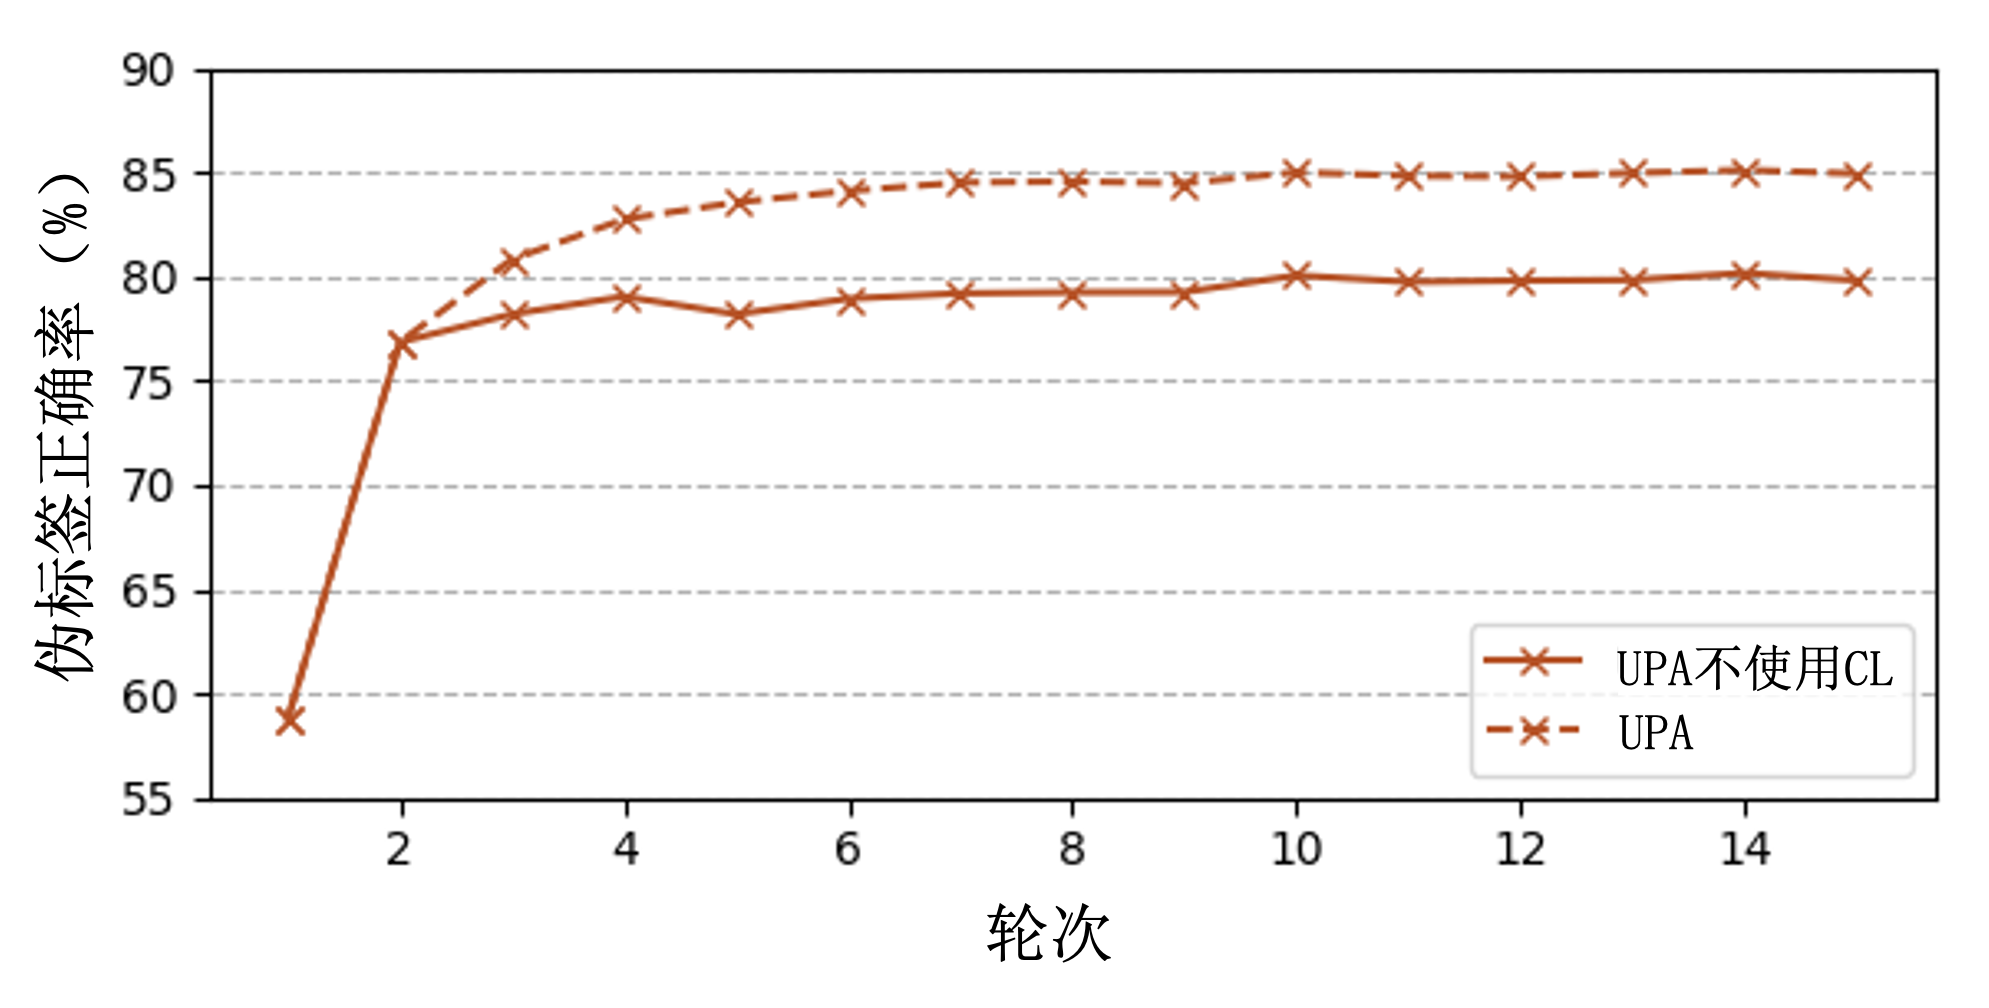
\includegraphics[width=0.55\linewidth]{figures/upa_extracted/cl_pl_acc.png}
  \bicaption[fig:upa_cl_acc]{}{UPA在 VisDA-C 数据集上所选伪标签精度的演化曲线}{Fig.}{Evolution of selected pseudo-label accuracy of UPA on VisDA-C}
\end{figure}

UPA 对四个核心超参数——置信样本筛选比例 $\gamma_{\text{sel}}$、对比温度 $\tau$、K 近邻数 $K$ 与损失权重 $\beta_{\text{CE}}$——在 $\pm 20\%$ 扰动范围内均保持稳定（如图~\ref{fig:param}）。具体而言：$\gamma_{\text{sel}}$ 在 0.5–0.9 范围内变化时，UPA 在 VisDA-C 与 Office 数据集上的精度波动不超过 1 个百分点，展现出良好的工程鲁棒性。$\tau$ 与 $K$ 的敏感性分析同样表明存在一个较宽的舒适区间，便于实际部署时调参。尽管 VisDA-C 数据集因域偏移更严重而对 $\gamma_{\text{sel}}$ 的选择更为敏感，UPA 在该数据集的默认参数设置下仍高于所有对比方法。

\begin{figure*}[!htbp]
  \centering
  \setlength{\tabcolsep}{0pt}
  \subfigure[置信样本筛选比例 $\gamma_{\text{sel}}$]{%
    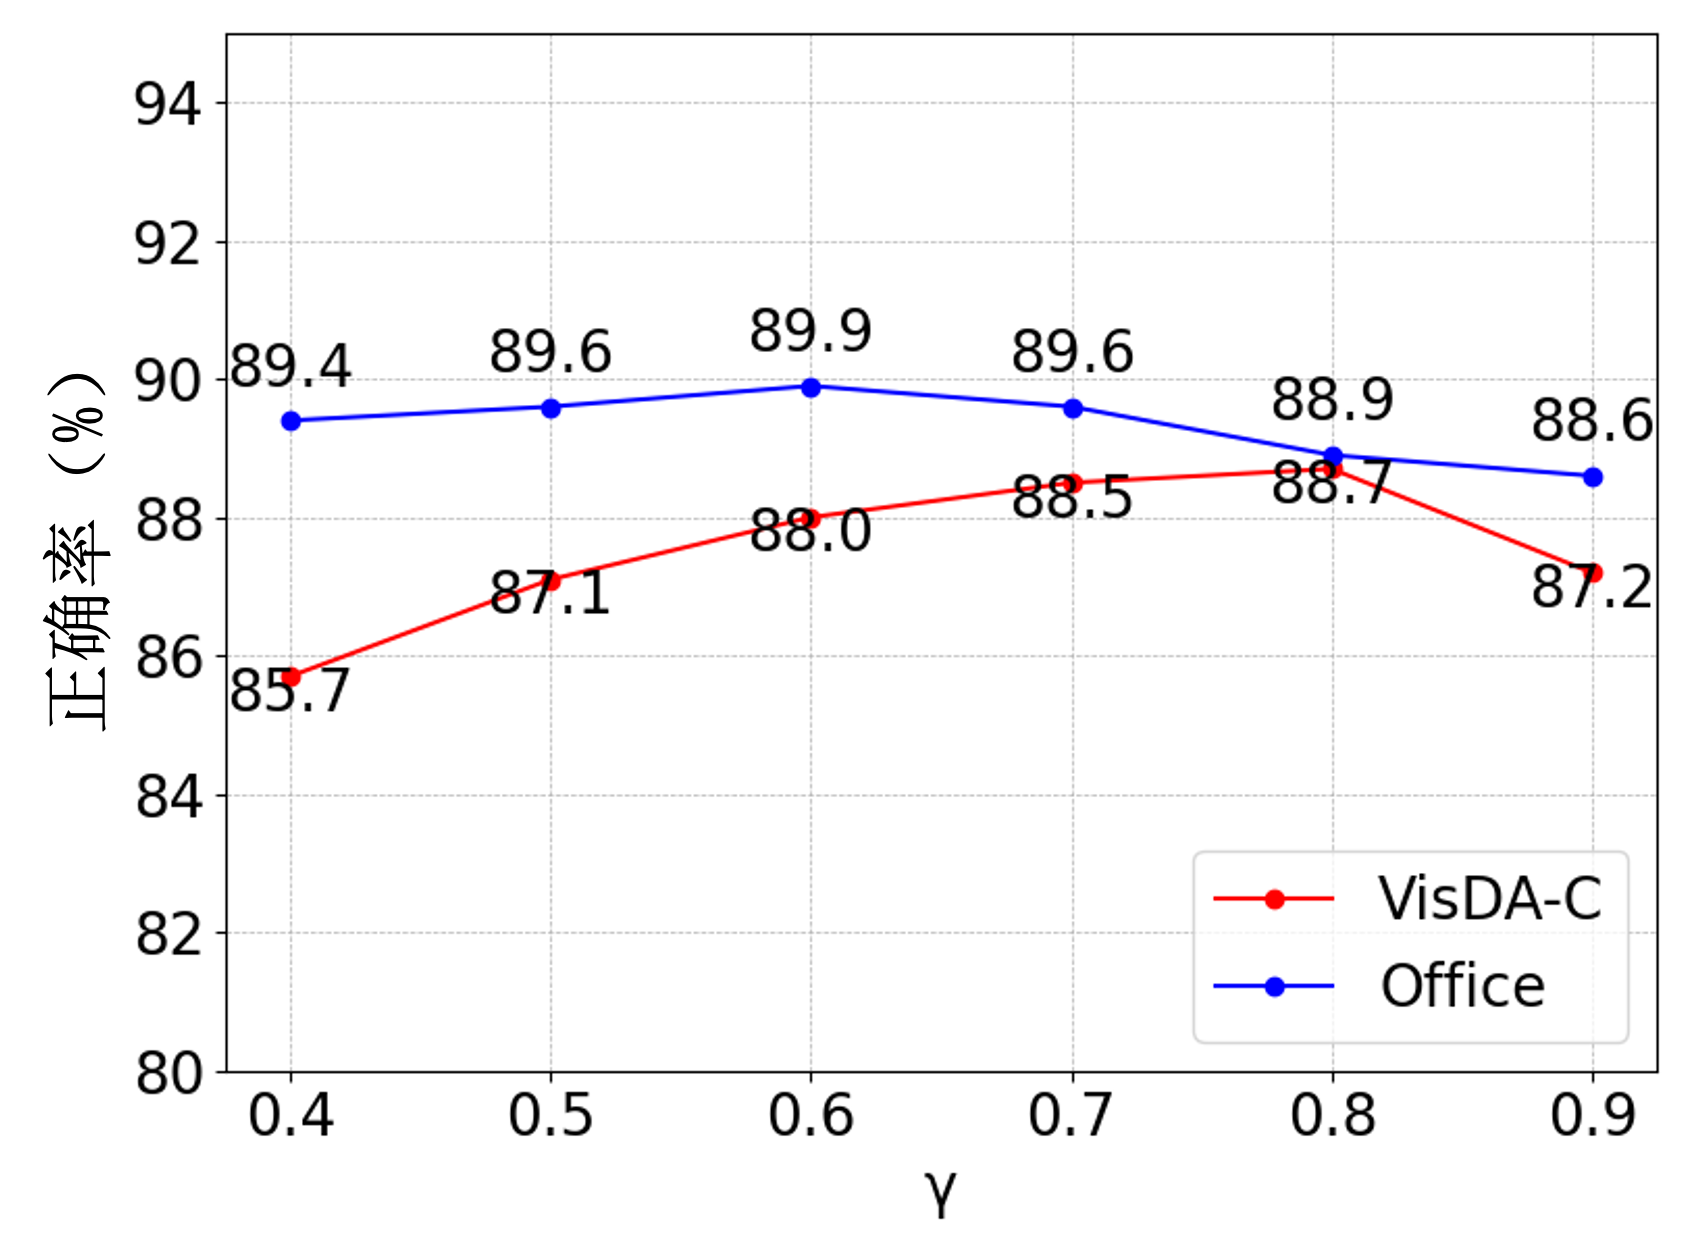
\includegraphics[width=0.3\linewidth]{figures/upa_extracted/re-sel_r_acc.png}
    \label{fig:param_gamma}%
  }\hfill
  \subfigure[对比温度 $\tau$]{%
    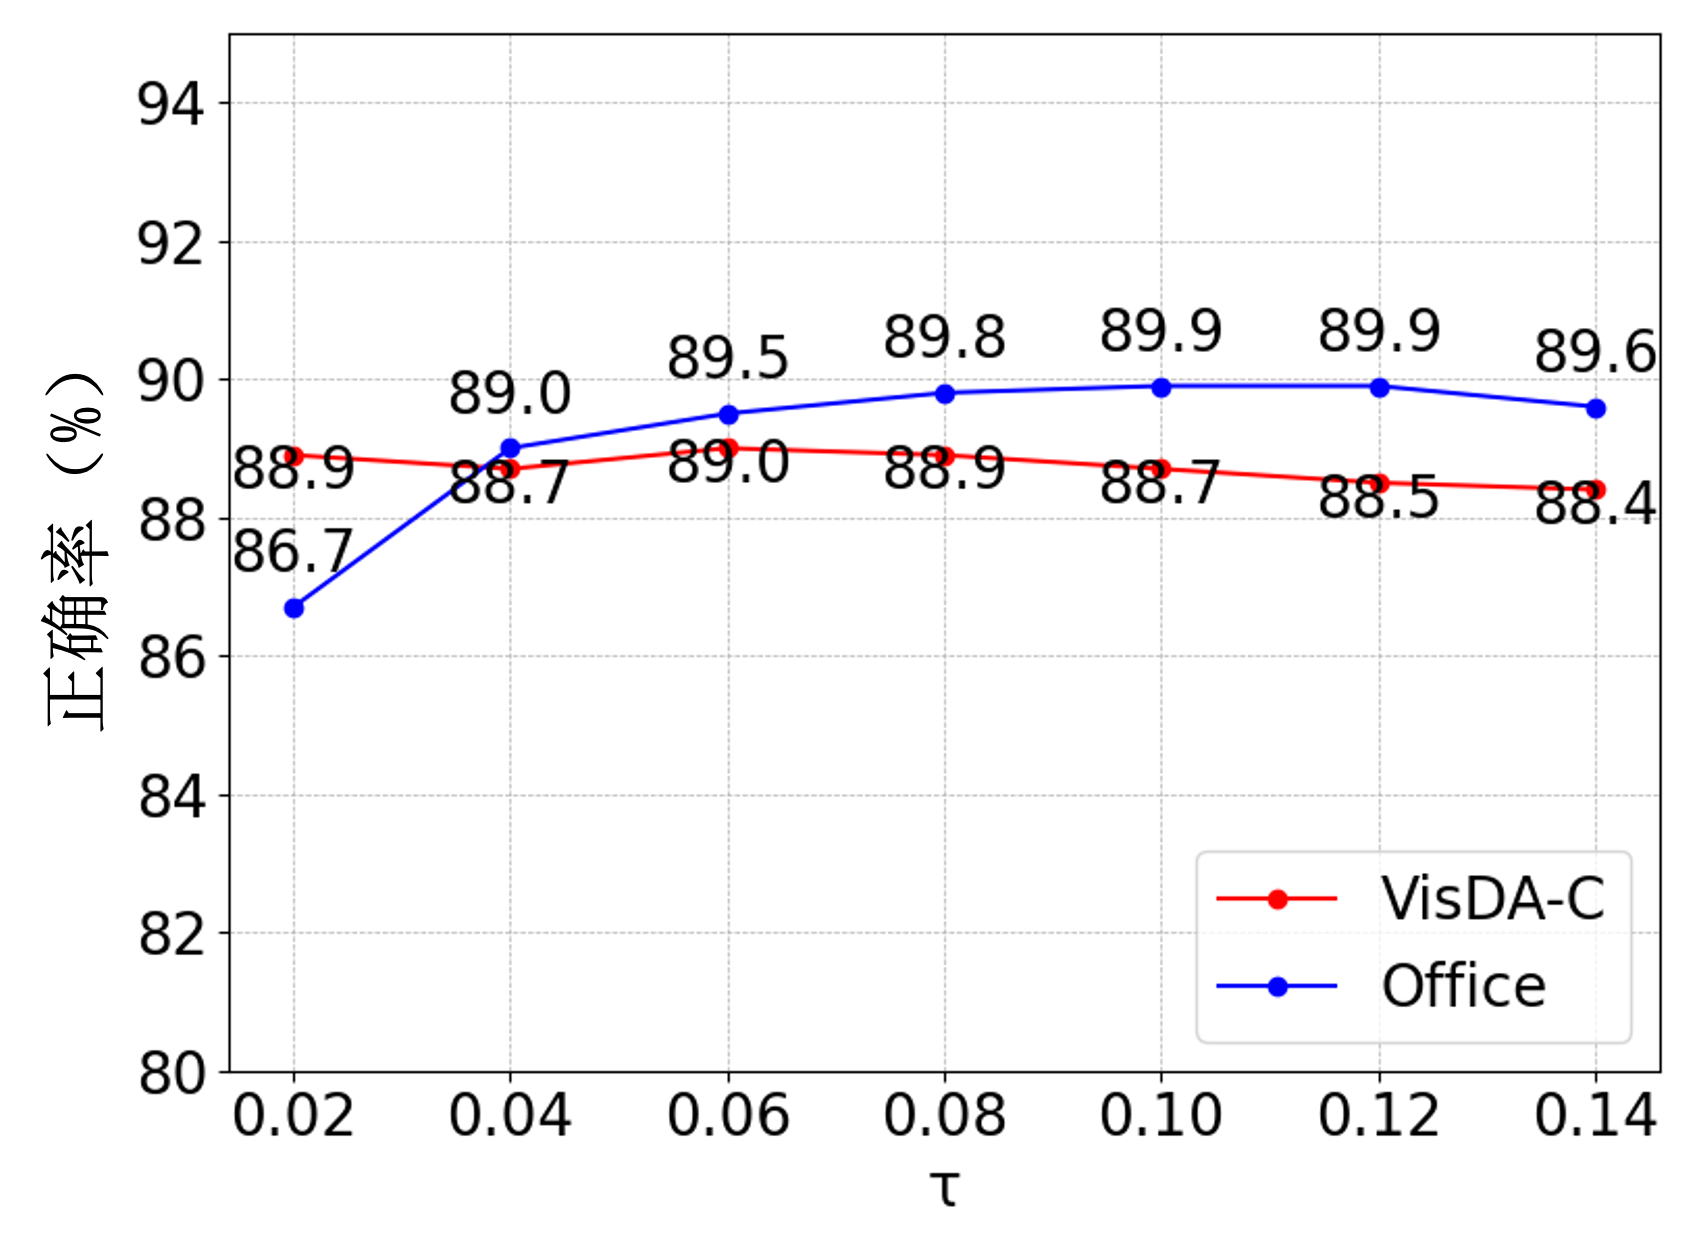
\includegraphics[width=0.3\linewidth]{figures/upa_extracted/re-tau_acc.png}
    \label{fig:param_tau}%
  }\hfill
  \subfigure[近邻数 $K$]{%
    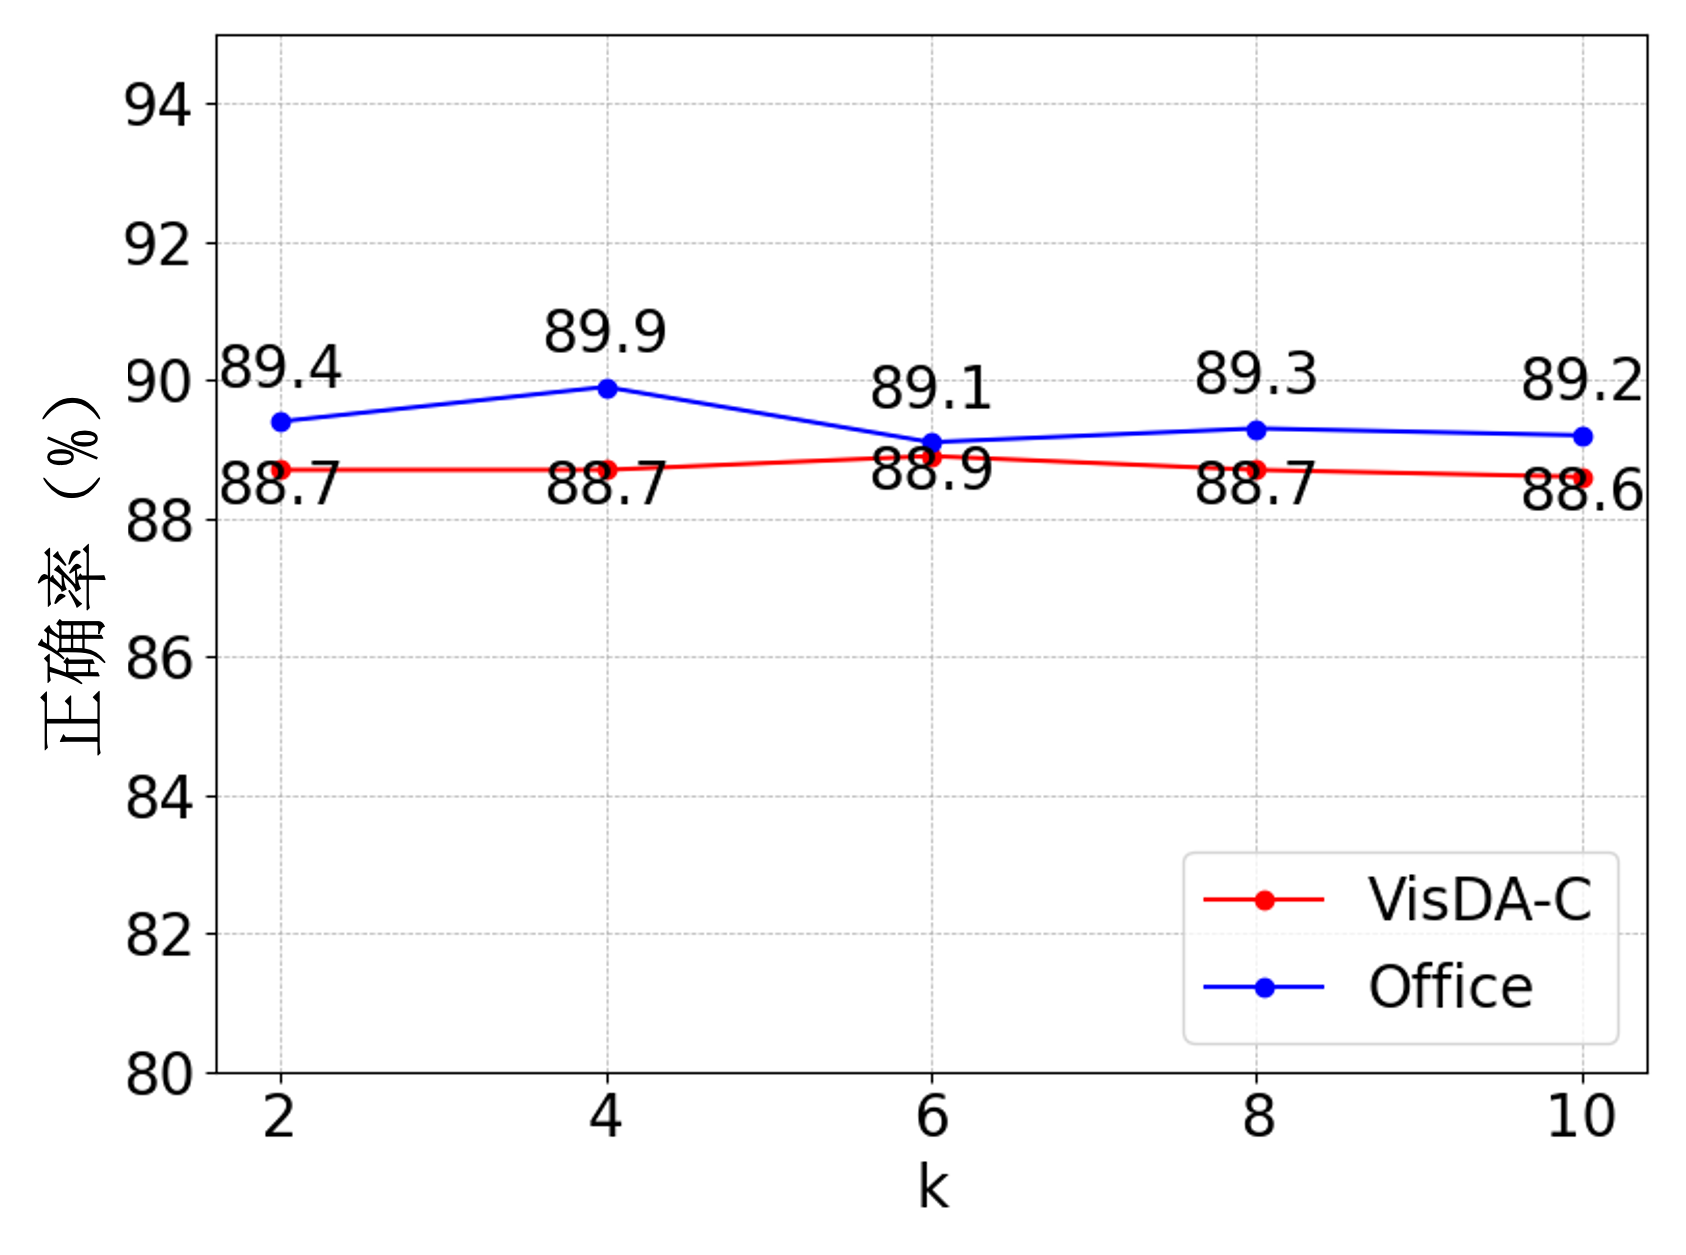
\includegraphics[width=0.3\linewidth]{figures/upa_extracted/re-k_acc.png}
    \label{fig:param_k}%
  }
  \bicaption[fig:param]{}{超参数敏感性分析}{Fig.}{Parameter sensitivity analysis on VisDA-C and Office datasets}
\end{figure*}

\newpage
\FloatBarrier
\noindent\textbf{(4) 可视化分析}

采用 t-SNE~\cite{van2008visualizing} 对 Office-Home 数据集 A$\to$P 任务的目标域特征进行可视化，如图~\ref{fig:upa_tsne}所示，左为源域特征；右为适应后目标域特征。结果表明，适应前，目标域特征与源域特征存在明显的域间差异，不同类别之间存在大量重叠；适应后（图~\ref{fig:upa_tsne} 右），域偏移显著减小，类内紧凑性与类间分离度均明显提升。CACL 的引入进一步细化了类边界，使得 APS 所选伪标签的精度得到持续保障。

\begin{figure}[!htbp]
    \centering
    \setlength{\tabcolsep}{0pt}
    \subfigure[]{%
      \includegraphics[width=0.48\linewidth]{papers/UPA/tsne_AP_class_source_box.pdf}
      \label{fig:tsne_source}%
    }\hfill
    \subfigure[]{%
      \includegraphics[width=0.48\linewidth]{papers/UPA/tsne_AP_class_target_box.pdf}
      \label{fig:tsne_target}%
    }
    \bicaption[fig:upa_tsne]{}{UPA的t-SNE 特征分布可视化}{Fig.}{t-SNE visualization of features}
\end{figure}

% \begin{figure}[!htbp]
%   \centering
%   \setlength{\tabcolsep}{0pt}
%   \subfigure[]{%
%     \includegraphics[width=0.48\linewidth]{papers/UPA/office-home_AP_acc_epoch.pdf}
%     \label{fig:curve_office}%
%   }\hfill
%   \subfigure[]{%
%     \includegraphics[width=0.48\linewidth]{papers/UPA/visda_acc_epoch.pdf}
%     \label{fig:curve_visda}%
%   }
%   \bicaption[fig:upa_curves]{}{UPA 在 A$\to$P（左）与 S$\to$R（右）任务上与 SHOT 基线的训练精度曲线对比}{Fig.}{Training accuracy curves of UPA vs. SHOT on A$\to$P (left) and S$\to$R (right) tasks, demonstrating UPA's faster convergence and higher final accuracy}
% \end{figure}

% \textbf{训练曲线分析} SHOT（不含 CACL）与 UPA（含完整 CACL）在 A$\to$P 与 S$\to$R 两个任务上的精度演进曲线（如图~\ref{fig:upa_curves}）显示：UPA 在训练初期即展现出更快的收敛速度与更高的收敛精度，约 10 个 epoch 内即可达到近似最优性能，且精度曲线平稳无显著波动。这一特性源于 APS 提供的可靠伪标签与 CACL 维护的类内语义一致性共同作用，有效避免了噪声标签导致的训练震荡。


\FloatBarrier

\section{基于选择性扫描的不确定性感知的迁移方法}

\label{sec:chap2_sfmamba}

UPA 从判别层去噪的角度抑制了伪标签噪声的累积，但其作用对象限于监督信号的可靠性，骨干自身的建模方式所引入的不确定性仍未被触及。为进一步控制跨域表征中的迁移不确定性，
本节在骨干网络层面引入状态空间模型 Mamba~\cite{gu2023mamba} 作为 SFDA 任务的骨干，并针对该骨干特有的表征层不确定性设计抑制机制。
Mamba定义了一类扫描序列到序列的映射，通过隐状态 $h(t) \in \mathbb{R}^N$ 将输入 $x(t)$ 映射为输出 $y(t)$，其状态转移参数是输入依赖的：$\Delta$、$B$、$C$ 均由当前输入 $x(t)$ 动态生成。连续时间常微分方程形式为：
\begin{equation}
h'(t) = A h(t) + B x(t), \quad y(t) = C h(t) + D x(t),
\label{eq:ssm_cont}
\end{equation}
其中 $A \in \mathbb{R}^{N \times N}$, $B \in \mathbb{R}^{N \times 1}$, $C \in \mathbb{R}^{1 \times N}$, $D \in \mathbb{R}$。离散化后形式化为：
\begin{equation}
h(t) = \overline{A} h(t-1) + \overline{B} x(t), \quad y(t) = C h(t) + D x(t).
\label{eq:ssm_disc}
\end{equation}

在视觉任务中，VMamba~\cite{liu2024vmamba} 将 Mamba 的序列建模扩展至二维图像，通过四向 2D 选择性扫描（沿行、列及对角线方向）捕获 patch 间的空间依赖关系。
这一性质使扫描过程承担了两项在视觉跨域场景中具有直接意义的功能。其一是长程依赖的线性聚合能力，状态 $h(t)$ 在时间维度上累积了此前全部位置的输入，因此相隔任意距离的两个 patch 之间仍存在直接的信息通路，这在 CNN 的固定局部感受野下并不存在；跨域偏移主要改变局部纹理统计而不改变图像的全局构成，长程依赖因此成为少数可跨域保持稳定的结构线索。其二是输入依赖的选择性，扫描状态可以依据当前输入的内容决定保留或跳过，从而抑制与判别无关的位置对状态演化的贡献。
% 据此，选择性扫描对跨域特征建模的作用可以解决“在何处聚合”与“聚合什么”两个可分离的问题。

% Mamba的关键改进是将时间尺度参数 $\Delta$ 与状态转移权重 $B$、$C$ 设计为输入序列 $x(t)$ 的动态函数，从而实现输入依赖的选择性扫描机制，使得 Mamba 能够在保持线性时间复杂度的同时，根据当前输入自适应调整状态转移行为。

与 CNN 骨干上迁移不确定性集中于判别层不同，Mamba 骨干下的迁移不确定性同时分布在表征层与序列层，构成其特有的双重不确定性问题：（1）表征层不确定性：VMamba 的选择性扫描主要沿空间维度展开，对跨通道频率域依赖建模不足~\cite{yang2020fda,qin2021fcanet}，如图~\ref{fig:cam_moti}，低频通道承载域不变的语义结构信息而高频通道更易受域差异干扰，源—目标域发生分布偏移时模型无法自适应强化语义稳定通道、抑制域敏感通道；（2）空间序列层不确定性：SSM 的隐藏状态演化依赖于输入序列的顺序，模型可能记忆源域扫描序列中前景与背景元素的空间共现模式（即“捷径学习”~\cite{geirhos2020shortcut}），如图~\ref{fig:scan}所示，当目标域打破这种空间配置时背景 patch 引入的虚假相关性会通过状态转移机制逐步累积放大，最终损害判别能力。这一序列层不确定性是 CNN 骨干上不存在、Mamba 序列建模独有的新风险。

\begin{figure}[!htbp]
  \centering
  \subfigure[ResNet101和VMamba-T的Grad-CAM可视化对比]{
    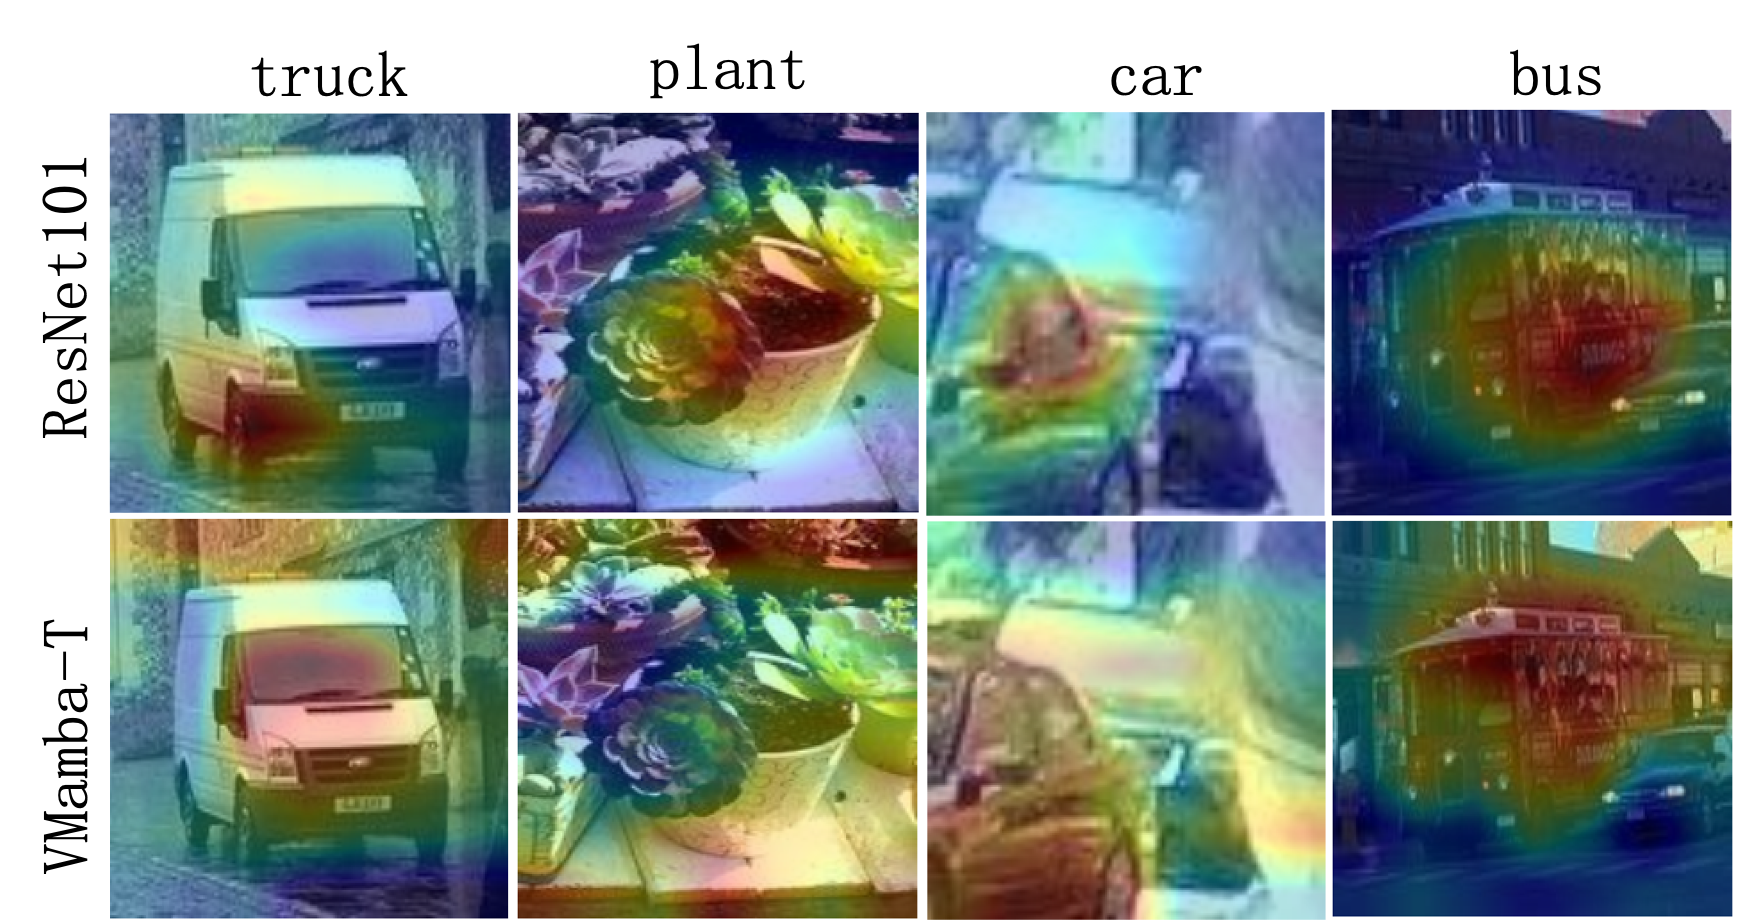
\includegraphics[width=0.48\textwidth]{figures/sfmamba/gradcam.png}
    \label{fig:cam_moti}
  }
  \hfill
  \subfigure[空间状态模型在域迁移下的错误预测传播阐述]{
    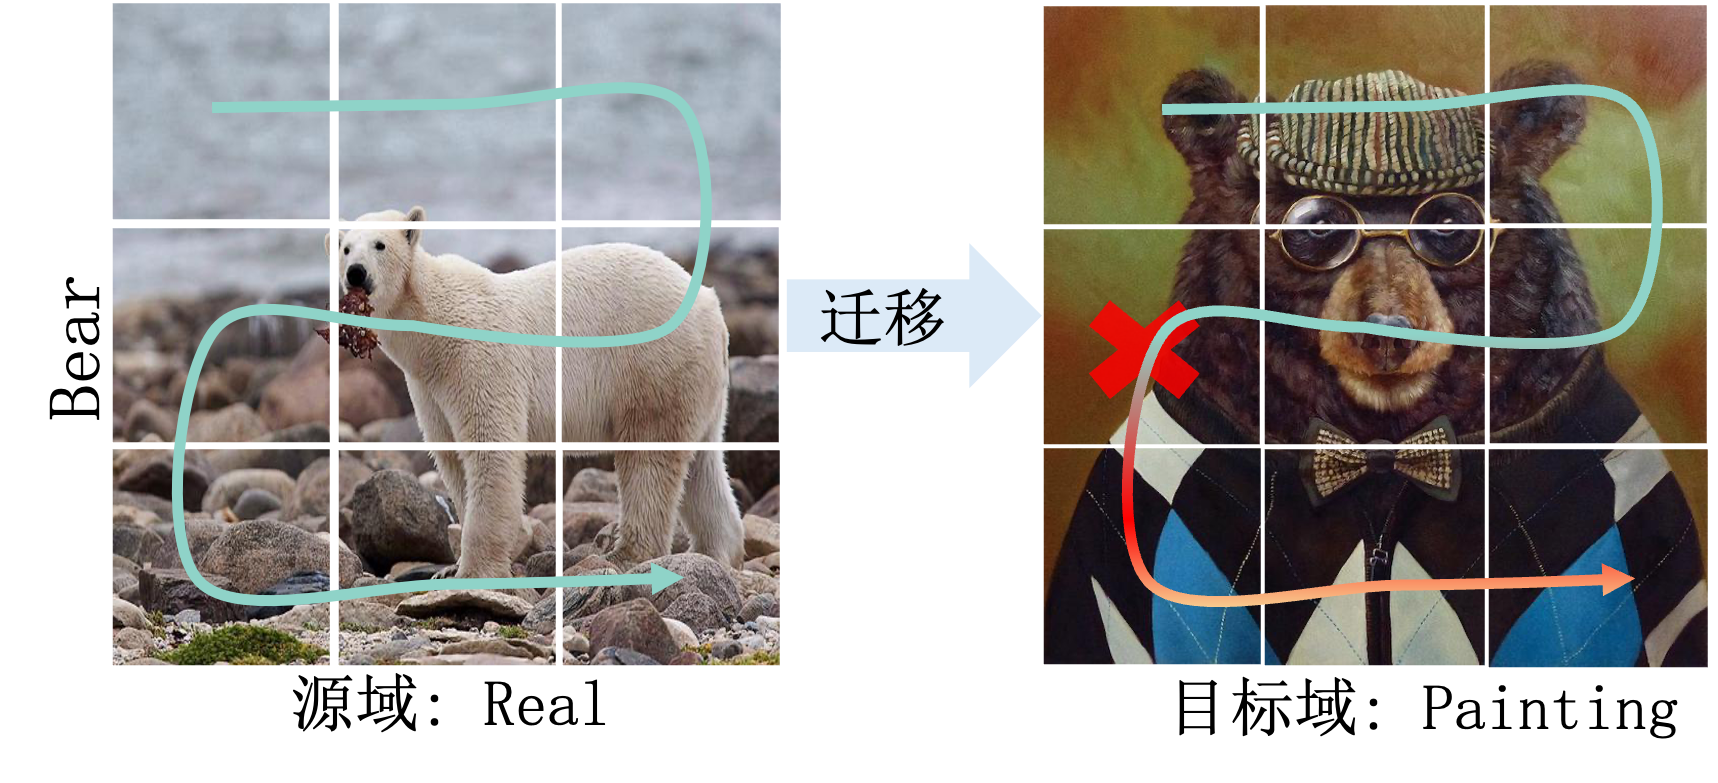
\includegraphics[width=0.48\textwidth]{figures/sfmamba/spatial_scanning.png}
    \label{fig:scan}
    }
    \bicaption[fig:sfmamba_uncertainty]{}{Mamba 骨干的迁移不确定性}{Fig.}{Transfer uncertainty of the Mamba backbone}
\end{figure}

本文提出SfMamba 针对上述两种不确定性分别设计抑制机制（图~\ref{fig:sfmamba_framework}）：通道级视觉状态空间模块（Channel-wise Visual State-Space, Ch-VSS）抑制表征层不确定性；语义一致性打乱策略抑制序列层不确定性。两条抑制路径共同实现对 SSM 骨干下迁移不确定性的协同治理。

\begin{figure}[!htbp]
    \centering
    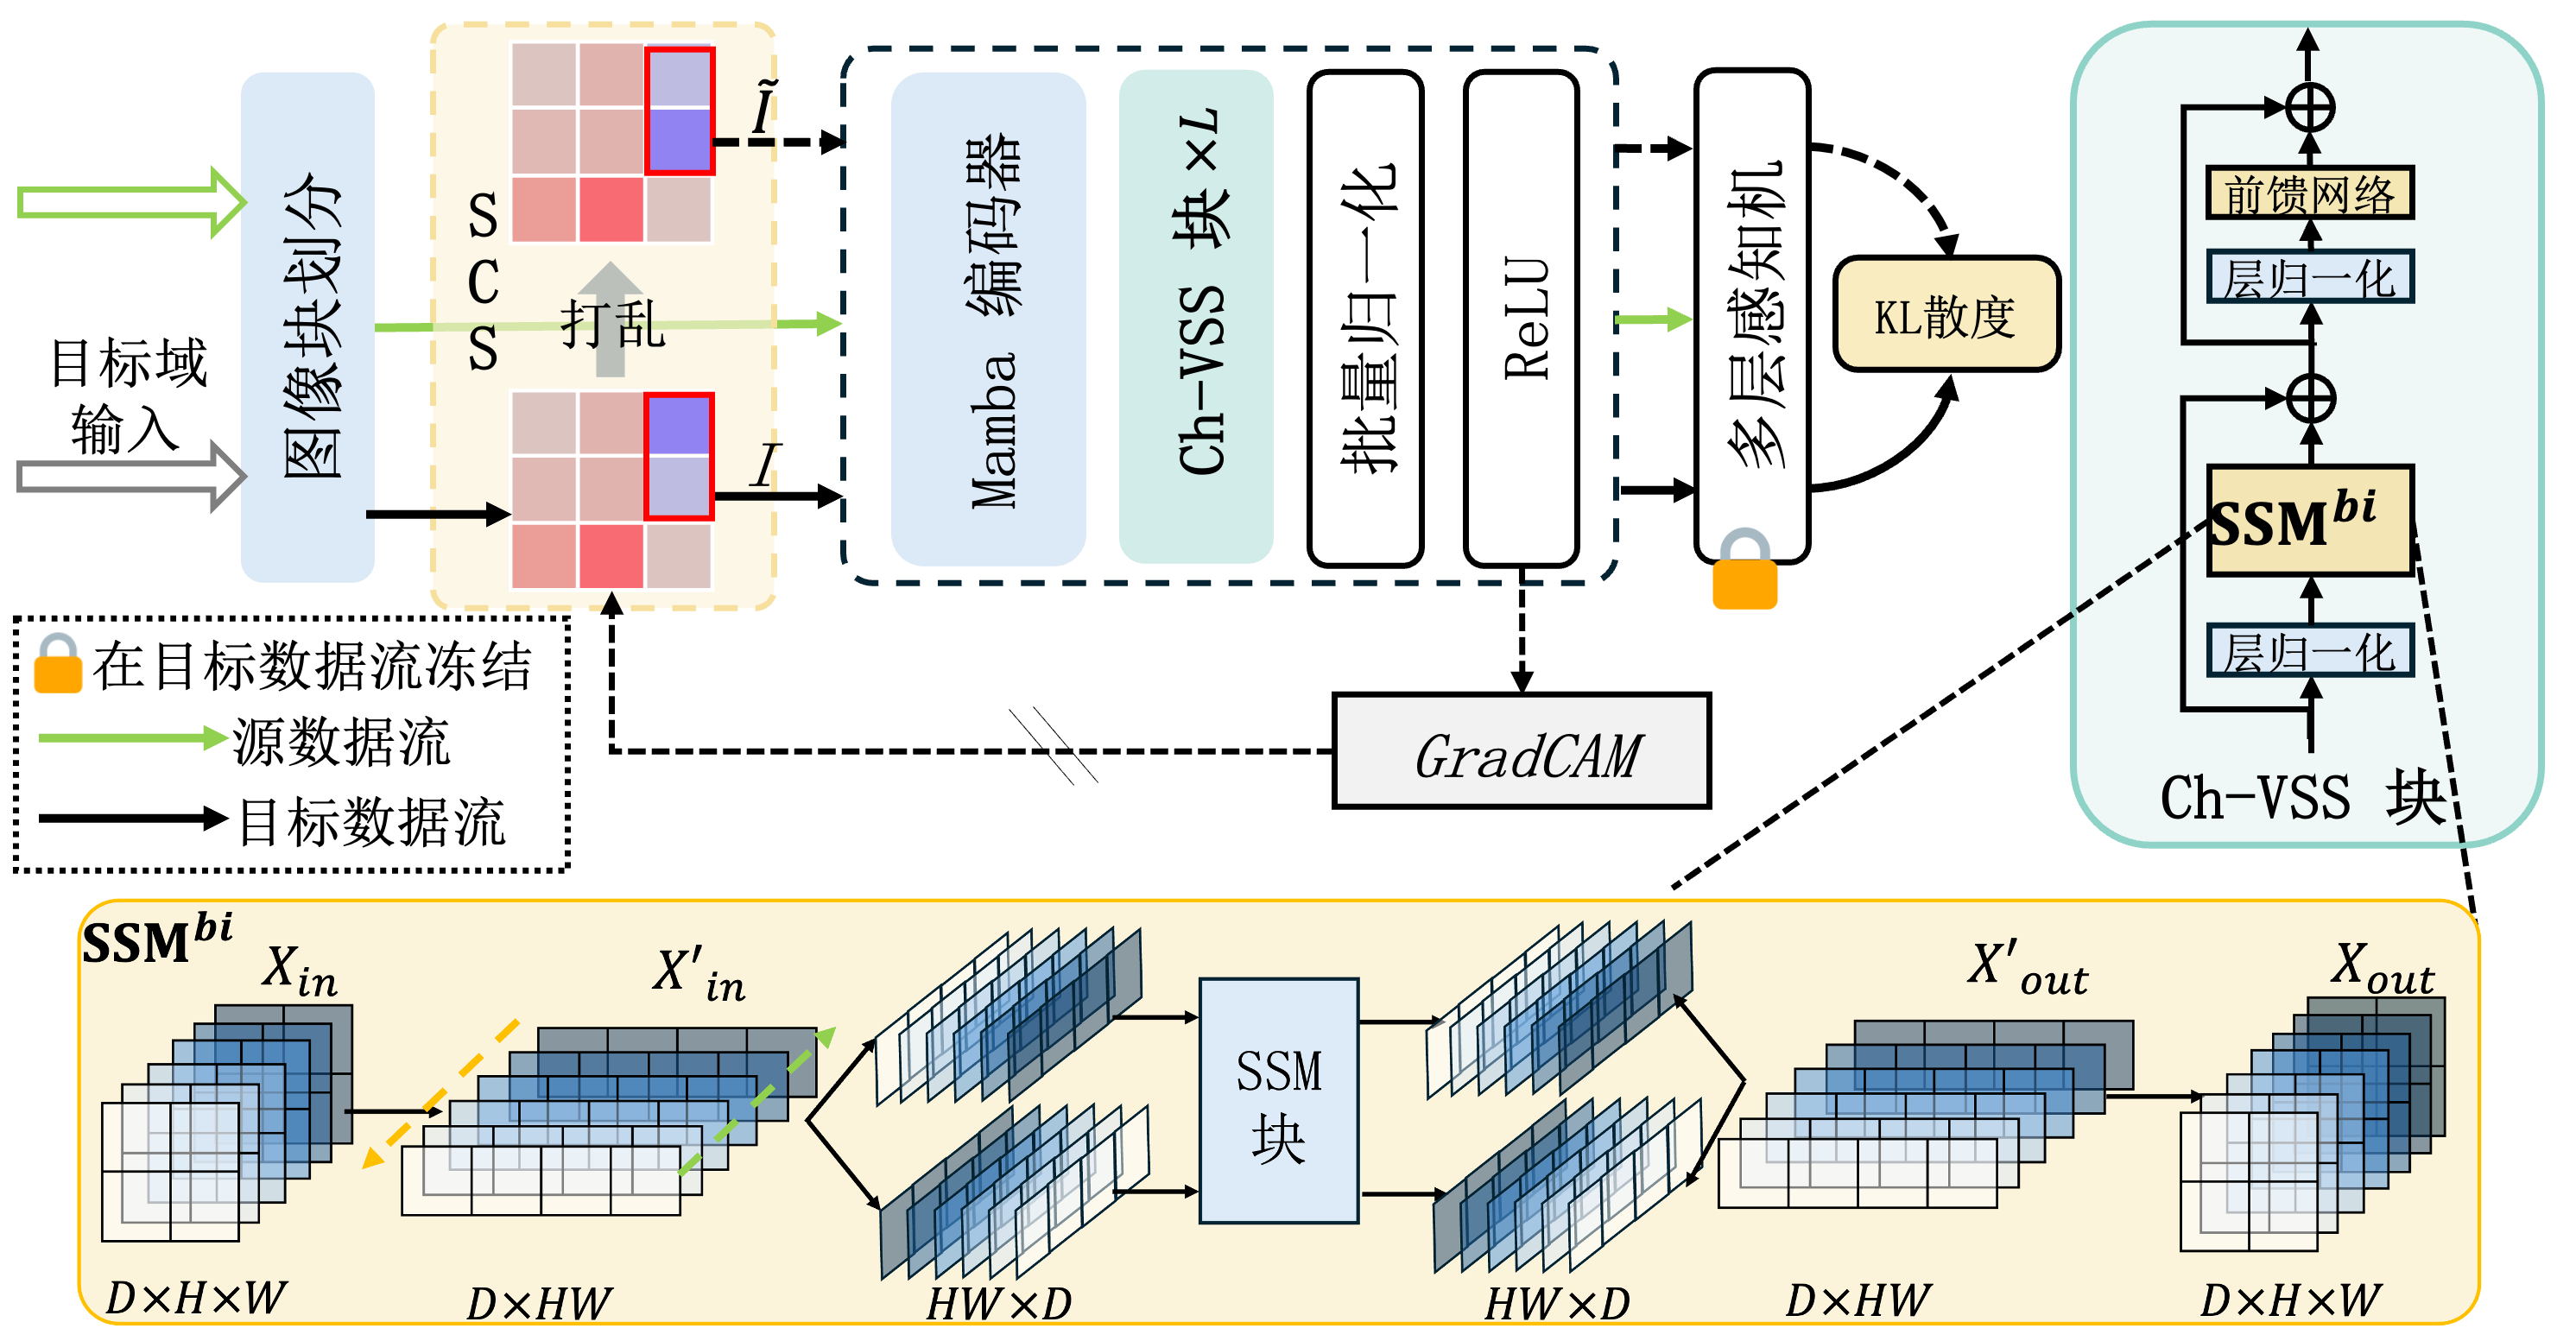
\includegraphics[width=0.95\textwidth]{figures/sfmamba/backbone.png}
    \bicaption[fig:sfmamba_framework]{}{SfMamba 总体框架}{Fig.}{Overview of SfMamba framework}
\end{figure}

\subsection{通道维度选择性扫描}

\label{sec:chap2_sfmamba_chvss}

视觉 VMamba 通过四向 2D 选择性扫描捕获 patch 间的空间长程依赖，但其在通道维度上的建模存在结构性短板：SSM 状态转移沿空间 token 顺序递归展开，每个时刻的状态更新仅与单一 patch 关联，跨通道频率域相关性需要等到所有空间 patch 完成扫描后通过后续通道投影间接获得，难以显式强化语义稳定的低频通道、抑制域敏感的高频通道。这一限制在源—目标域发生显著分布偏移时尤为突出：低频通道承载的跨域一致纹理与轮廓信息与高频通道承载的域特异细节在适应阶段出现响应失衡，而现有 SSM 骨干下的通道建模工作多在复杂的层级框架内引入通道注意力以提升特定任务（图像重建、源数据可访问的目标检测）的性能，鲜有针对 SFDA 设定下“骨干固定 + 无源数据参与”约束设计的轻量级通道选择性机制。

% \textbf{与现有通道注意力工作的对比} 主流方案与 SfMamba 的核心差异在于对源数据与骨干修改的依赖度不同（如图~\ref{fig:sfmamba_chvss_compare}）：一些方法在多层重建框架内集成通道注意力以服务于图像重建任务，未针对分类任务的判别层迁移去噪进行适配；另一些方法通过域间通道混合实现跨域对齐，但强制要求源域与目标域数据在适应阶段同时可用，违背 SFDA 的“无源”约束。SfMamba 的 Ch-VSS 模块则采取显式的通道维度双向扫描策略，将通道相关性建模为可学习的基础特征重组策略，既不修改源骨干参数也不要求源数据参与，与 SFDA 设定完全契合。

\begin{figure}[!htbp]
    \centering
    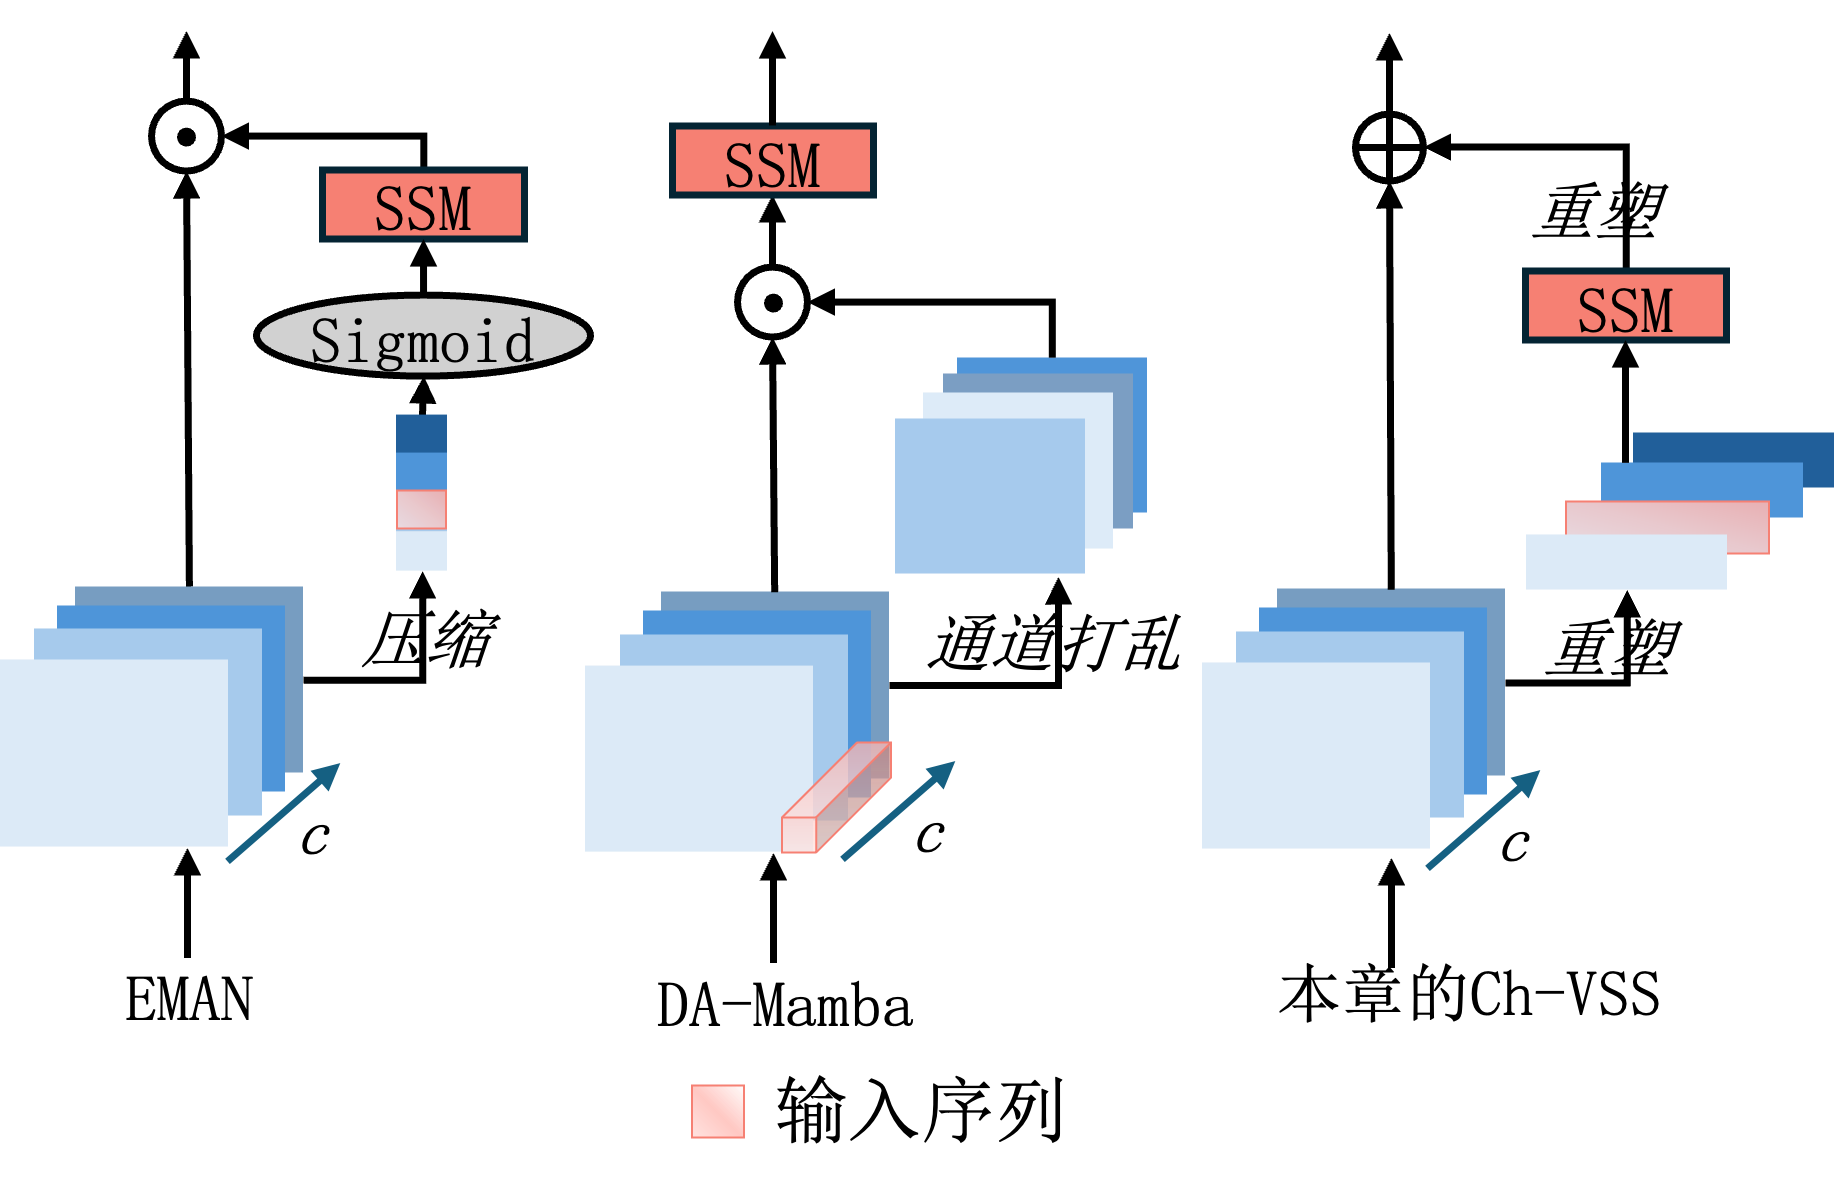
\includegraphics[width=0.6\linewidth]{figures/sfmamba/mamba_channel_atten.png}
    \bicaption[fig:sfmamba_chvss_compare]{}{Mamba 骨干上通道维度注意力机制对比示意}{Fig.}{Comparison of channel-wise attention mechanisms integrated on the Mamba backbone}
\end{figure}

给定骨干网络特征图 $X_{\text{in}} = g(x^t) \in \mathbb{R}^{D \times H \times W}$，Ch-VSS 首先将其重塑为通道向量序列 $X'_{\text{in}} \in \mathbb{R}^{D \times (HW)}$，然后沿通道维度应用双向 SSM，以缓解单向扫描带来的通道顺序偏置：
\begin{align}
    X'_{\rightarrow} &= \text{SSM}(X'_{\text{in}}), \quad
    X'_{\leftarrow} = \text{SSM}\!\big(\textit{Reverse}(X'_{\text{in}})\!\big), \notag \\
    X'_{\text{out}} &= \text{SSM}_{\text{bi}}(X'_{\text{in}}) = X'_{\leftarrow} + \textit{Reverse}(X'_{\rightarrow}) \in \mathbb{R}^{D \times (HW)},
    \label{eq:ch_scan}
\end{align}
其中正向扫描沿 $1 \rightarrow D$ 方向聚合通道信息，反向扫描沿 $D \rightarrow 1$ 方向聚合，最终通过融合两侧响应获得与通道顺序无关的全局依赖。处理后的序列被重塑回特征图 $X_{\text{out}} \in \mathbb{R}^{D \times H \times W}$，并通过残差连接与原始特征相加以保留骨干网络的空间结构信息。Ch-VSS 整体作为辅助 neck 网络嵌入模型末端，可形式化为：
\begin{equation}
    \theta_t(x^t) = f\!\left(\text{Ch-VSS}\!\big(g(x^t)\big)\right).
    \label{eq:sf_chvss_out}
\end{equation}

通道维度扫描对表征层不确定性的抑制体现在两个方面：（1）双向通道扫描直接建模跨通道的频率域相关性，使模型自适应强化语义稳定的低频通道、抑制域敏感的高频通道；（2）通道扫描捕获跨域一致的基础模式（如边缘检测器、纹理基元），这些模式在源—目标域分布偏移下保持稳定，从而构成“域不变基础特征”。

% Ch-VSS 本质上学习的是一种“通道维度的特征重组策略”，即通过双向通道扫描建立不同频率域通道之间的关联模式。这种关联模式需要在源域数据上进行充分的监督学习才能稳定建立。实验表明：仅在目标域适应阶段引入随机初始化或零初始化~\cite{zhang2023adding} 的 Ch-VSS 相比基线无显著改善，验证了源域预训练是 Ch-VSS 发挥表征层不确定性抑制作用的必要前提。

\subsection{空间2D选择性扫描}

\label{sec:chap2_sfmamba_scs}

为抑制空间2D维度 SSM 序列建模中的虚假相关累积，本文提出了语义一致性打乱（Semantic-Consistent Shuffle, SCS）策略。SCS 的核心思想是：通过打乱背景 patch 的顺序打破虚假的空间相关性，同时通过一致性正则迫使模型在不依赖空间配置的情况下维持预测。

SCS 在 patch 粒度上操作。沿用 VMamba 的 patch 嵌入向量设定，特征图被划分为大小 $p \times p$、步长 $p$ 的非重叠 patch，对于空间分辨率 $H \times W$ 的特征图，共产生 $N_p = (H/p) \times (W/p)$ 个 patch token。GradCAM~\cite{selvaraju2017grad} 在骨干网络末端层生成的激活图谱被重采样至 patch 分辨率，并在每个 patch 区域内聚合为一个 patch 级别的重要性得分。基于此得分，识别相对于伪标签 $\hat{y}$ 激活值最低的 $\gamma_{\text{bg}}\%$ 的 patch 作为背景 patch 集合 $\{P_k\}_{k=1}^{N_p}$。这些背景 patch 在源域中往往与目标对象存在稳定的共现关系，是空间捷径学习的主要载体。
所以本文通过随机置换矩阵 $\Pi$ 对背景 patch 进行重排：
\begin{equation}
\tilde{P}_k = P_{\Pi(k)}, \quad \tilde{U} = \text{Replace}(U, \{\tilde{P}_k\}),
\label{eq:shuffle}
\end{equation}
得到扰动序列 $\tilde{U}$。该操作在 VMamba 的四条 2D 扫描路径（沿行、列、两条对角线方向）上均会破坏固定的上下文关系（如图~\ref{fig:sfmamba_scs_compare}），使模型无法再依赖“前景—背景”空间共现进行预测，从根源上切断序列层迁移不确定性的累积链路。

\begin{figure}[!htbp]
    \centering
    \includegraphics[width=0.7\linewidth]{papers/Sfmamba/scs.pdf}
    \bicaption[fig:sfmamba_scs_compare]{}{SCS 策略描述图}{Fig.}{The illustration of the SCS strategy}
\end{figure}

为保证打乱操作不损害模型对前景语义的判别能力，引入 KL 散度一致性正则：
\begin{equation}
\mathcal{L}_{\text{KL}} = \mathbb{E}_{x^t \sim \mathcal{T}} D_{\text{KL}}\!\left(\theta_t(U) \,\|\, \theta_t(\tilde{U})\right),
\label{eq:kl_loss}
\end{equation}
迫使模型在原始序列与打乱序列上的输出分布保持一致。这一约束使 SSM 的隐藏状态演化主要依赖鲁棒的前景特征，而非背景序列的顺序，从而抑制 SSM 序列建模独有的序列层迁移不确定性。

% \subsection{邻居感知去噪与总体训练流程}
% \label{sec:chap2_sfmamba_training}

为缓解伪标签噪声对 $\mathcal{L}_{\text{CE}}$ 与 $\mathcal{L}_{\text{KL}}$ 的负面影响，SfMamba 沿用§\ref{sec:chap2_upa_denoising}提出的邻居感知去噪策略作为子组件：对每个目标样本 $x^t$ 构建 K 近邻集合 $\mathcal{N}_t$ 并迭代估计精炼伪标签 $\hat{y}'$ 与置信度评分 $q_t$，按类别内排序选取前 $\gamma_{\text{sel}}\%$ 样本构成高质量子集 $\mathcal{T}_c$，仅在该子集上计算 $\mathcal{L}_{\text{CE}}$ 与 $\mathcal{L}_{\text{KL}}$：
\begin{equation}
\mathcal{L}_{\text{CE}} = -\mathbb{E}_{x^t \in \mathcal{T}_c} \sum_{c=1}^{C} \hat{y}_c \log p_c(x^t), \quad
\mathcal{L}_{\text{KL}} = \mathbb{E}_{x^t \in \mathcal{T}_c} D_{\text{KL}}\!\left(\theta_t(U) \,\|\, \theta_t(\tilde{U})\right).
\label{eq:scs_loss_ch}
\end{equation}

最终，SfMamba 的总体训练损失为：
\begin{equation}
\mathcal{L} = \mathcal{L}_{\text{KL}} + \mathcal{L}_{\text{ent}} + \mathcal{L}_{\text{div}} + \mathcal{L}_{\text{CE}},
\label{eq:scs_total_loss}
\end{equation}
其中 $\mathcal{L}_{\text{ent}}$ 与 $\mathcal{L}_{\text{div}}$ 的形式化参见式~\eqref{eq:chap2_im}。

% 整体训练沿用 §2.3 APS 框架的迭代式伪标签精炼—损失更新循环，体现两条方法路线在抑制判别层不确定性上的模块级可组合性。两路径对迁移不确定性的整体抑制结构可总结为：UPA 以邻居一致性提供判别层去噪，SfMamba 在其基础上以 Ch-VSS 抑制表征层不确定性、以 SCS 抑制序列层不确定性，三层叠加形成对迁移不确定性的协同抑制。

\subsection{实验结果与分析}

\noindent\textbf{(1) 数据集与实验设置}

本节同样在 Office~\cite{saenko2010adapting}、Office-Home~\cite{venkateswara2017deep}、VisDA-C~\cite{peng2017visda} 与 DomainNet-126~\cite{saito2019semi}四个广泛使用的 SFDA 基准上评估 SfMamba。
% 具体而言：Office 数据集包含 Amazon（A）、Dslr（D）与 Webcam（W）三个域；Office-Home 数据集包含 Art（Ar）、Clipart（C）、Product（P）与 Real World（R）四个域，共 65 个子域迁移任务；VisDA-C 数据集包含合成域 Synthetic（S）与真实域 Real（R）的跨域分割任务；DomainNet-126 包含 Real（R）、Painting（P）、Clipart（C）与 Sketch（S）四个域。
SfMamba 采用 VMamba-T（Tiny）与 VMamba-S（Small）两种规模的 SSM 骨干，并以 SHOT~\cite{liang2021source} 自训练框架为基础，冻结分类器。

SfMamba 采用 AdamW 优化器，权重衰减率为$5 \times 10^{-2}$，并用余弦退火策略，批次大小为 32，在单卡 NVIDIA RTX A100 GPU进行实验。源域预训练 Office/Office-Home/VisDA-C/DomainNet-126 分别为 100/50/10/30 个 epoch，目标域适应阶段背景比例 $\gamma_{\text{bg}} = 20\%$，所有结果报告三次随机种子 $\{0, 1, 2\}$ 的平均值。



\begin{table}[!htbp]
  \bicaption[tab:main_oh_visda]{}{SfMamba 在 Office-Home 与 VisDA-C 数据集上的准确率对比}{Table}{SfMamba accuracy on Office-Home and VisDA-C}
  \vspace{0.5em}\centering\wuhao
  \setlength{\tabcolsep}{1pt}
  \resizebox{\textwidth}{!}{
  \begin{tabular}{lc*{13}{c}c}
  \toprule
  \multirow{2}*{方法} & \multirow{2}*{SF} & \multicolumn{13}{c}{Office-Home} & \multicolumn{1}{c}{VisDA-C} \\
  \cline{3-16}
  & & A$\rightarrow$C & A$\rightarrow$P & A$\rightarrow$R & C$\rightarrow$A & C$\rightarrow$P & C$\rightarrow$R & P$\rightarrow$A & P$\rightarrow$C & P$\rightarrow$R & R$\rightarrow$A & R$\rightarrow$C & R$\rightarrow$P & Avg & S$\rightarrow$R \\
  \midrule
  \multicolumn{16}{c}{\textit{基于CNN的方法}} \\
  \midrule
  ResNet~\cite{he2016deep} & \checkmark & 44.0 & 65.9 & 74.0 & 52.1 & 61.0 & 65.4 & 52.2 & 40.9 & 72.9 & 64.1 & 45.3 & 77.9 & 59.6 & 47.8 \\
  SHOT~\cite{liang2021source} & \checkmark & 57.1 & 78.1 & 81.5 & 68.0 & 78.2 & 78.1 & 67.4 & 54.9 & 82.2 & 73.3 & 58.8 & 84.3 & 71.8 & 82.9 \\
  % NRC~\cite{yang2021neighbor} & \checkmark & 57.7 & 80.3 & 82.0 & 68.1 & 79.8 & 78.6 & 65.3 & 56.4 & 83.0 & 71.0 & 58.6 & 85.6 & 72.2 & 85.9 \\
  % CoWA-JMDS~\cite{cowa} & \checkmark & 56.9 & 78.4 & 81.0 & 69.1 & 80.0 & 79.9 & 67.7 & 57.2 & 82.4 & 72.8 & 60.5 & 84.5 & 72.5 & 86.9 \\
  NAMI~\cite{zhang2024neighborhood} & \checkmark & 58.3 & 80.9 & 82.9 & 68.5 & 80.5 & 79.6 & 66.0 & 57.0 & 83.7 & 71.9 & 59.9 & 85.0 & 72.9 & 88.9 \\
  UPA  & \checkmark & 57.3 & 79.5 & 82.4 & 68.2 & 81.0 & 80.2 & 69.3 & 55.4 & 82.3 & 75.3 & 59.2 & 85.5 & 73.0 & 88.7 \\
  % TPWA~\cite{tpwa} & \checkmark & 58.8 & 80.3 & 82.4 & 69.5 & 80.6 & 78.8 & 68.4 & 55.8 & 82.0 & 74.7 & 59.2 & 85.5 & 73.0 & 87.2 \\
  % SHOT+DPC~\cite{dpc} & \checkmark & 59.2 & 79.8 & 82.6 & 68.9 & 79.7 & 79.5 & 68.6 & 56.5 & 82.9 & 73.9 & 61.2 & 85.4 & 73.2 & 84.3 \\
  I-SFDA~\cite{mitsuzumi2024understanding} & \checkmark & 60.7 & 78.9 & 82.0 & 69.9 & 79.5 & 79.7 & 67.1 & 58.8 & 82.3 & 74.2 & 61.3 & 86.4 & 73.4 & 88.4 \\
  % C-SFDA~\cite{karim2023c} & \checkmark & 60.3 & 80.2 & 82.9 & 69.3 & 80.1 & 78.8 & 67.3 & 58.1 & 83.4 & 73.6 & 61.3 & 86.3 & 73.5 & 87.8 \\
  % TPDS~\cite{tang2023tpds} & \checkmark & 59.3 & 80.3 & 82.1 & 70.6 & 79.4 & 80.9 & 69.8 & 56.8 & 82.1 & 74.5 & 61.2 & 85.3 & 73.5 & 87.6 \\
  % DPL~\cite{xia2024dual} & \checkmark & 60.9 & 80.8 & 82.3 & 69.9 & 79.5 & 80.0 & 70.0 & 57.0 & 82.7 & 75.7 & 63.0 & 86.0 & 74.0 & 87.8 \\
  RGV~\cite{zhu2025revisiting} & \checkmark & 61.2 & 80.9 & 82.7 & 69.3 & 81.2 & 81.4 & 68.1 & 58.8 & 83.4 & 74.6 & 62.4 & 85.7 & 74.1 & \underline{89.1} \\
  DAPL~\cite{ge2023domain} & \ding{55} & 54.1 & 84.3 & 84.8 & 74.4 & 83.7 & 85.0 & 74.5 & 54.6 & 84.8 & 75.2 & 54.7 & 83.8 & 74.5 & 86.9 \\
  \midrule
  \multicolumn{16}{c}{\textit{基于ViT的方法}} \\
  \midrule
  DeiT-S~\cite{deit} & \checkmark & 55.6 & 73.0 & 79.4 & 70.6 & 72.9 & 76.3 & 67.5 & 51.0 & 81.0 & 74.5 & 53.2 & 82.7 & 69.8 & - \\
  DeiT-B~\cite{deit} & \checkmark & 61.8 & 79.5 & 84.3 & 75.4 & 78.8 & 81.2 & 72.8 & 55.7 & 84.4 & 78.3 & 59.3 & 86.0 & 74.8 & 67.1 \\
  CDTrans-S~\cite{xu2022cdtrans} & \ding{55} & 60.6 & 79.5 & 82.4 & 75.6 & 81.0 & 82.3 & 72.5 & 56.7 & 84.4 & 77.0 & 59.1 & 85.5 & 74.7 & - \\
  SHOT-B~\cite{liang2021source} & \checkmark & 67.1 & 83.5 & 85.5 & 76.6 & 83.4 & 83.7 & 76.3 & 65.3 & 85.3 & 80.4 & 66.7 & 83.4 & 78.1 & 83.5 \\
  CDTrans-B~\cite{xu2022cdtrans} & \ding{55} & 68.8 & \underline{85.0} & 86.9 & \underline{81.5} & \underline{87.1} & \underline{87.3} & \underline{79.6} & 63.3 & \underline{88.2} & 82.0 & 66.0 & \underline{90.6} & 80.5 & 88.4 \\
  DSiT-B~\cite{sanyal2023domain} & \checkmark & 69.2 & 83.5 & 87.3 & 80.7 & 86.1 & 86.2 & 77.9 & \underline{67.9} & 86.6 & 82.4 & 68.3 & 89.8 & 80.5 & 87.6 \\
  C-SFTrans~\cite{sanyal2024aligning} & \checkmark & \underline{70.3} & 83.9 & 87.3 & 80.2 & 86.9 & 86.1 & 78.9 & 65.0 & 87.7 & \underline{82.6} & 67.9 & 90.2 & 80.6 & 88.3 \\
  \midrule
  \multicolumn{16}{c}{\textit{基于Mamba的方法}} \\
  \midrule
  Source-T & \checkmark & 59.0 & 76.8 & 83.0 & 69.8 & 76.5 & 78.2 & 68.9 & 54.6 & 82.4 & 74.8 & 58.3 & 85.4 & 72.3 & 61.5 \\
  Source-S & \checkmark & 62.9 & 79.5 & 84.7 & 74.4 & 80.2 & 81.2 & 71.9 & 56.9 & 84.4 & 78.4 & 61.9 & 86.6 & 75.3 & 65.6 \\
  SHOT-T$^\dagger$~\cite{liang2021source} & \checkmark & 64.9 & 80.1 & 83.6 & 75.4 & 81.4 & 81.3 & 71.7 & 60.7 & 84.9 & 77.4 & 66.1 & 87.7 & 76.3 & 81.9 \\
  SHOT-S$^\dagger$~\cite{liang2021source} & \checkmark & 67.3 & 81.5 & 85.6 & 79.9 & 85.3 & 83.8 & 76.1 & 66.4 & 85.3 & 80.1 & 69.0 & 88.7 & 79.1 & 84.6 \\
  SfMamba-T & \checkmark & 67.5 & 80.9 & 87.4 & 77.6 & 83.4 & 86.4 & 76.2 & 66.1 & 86.9 & 78.7 & \underline{69.6} & 89.8 & 79.2 & 88.5 \\
  DATMamba~\cite{gao2025datmamba} & \checkmark & 67.1 & \textbf{86.3} & \underline{87.8} & \textbf{81.7} & \textbf{87.3} & 85.4 & \textbf{80.2} & 66.3 & 87.1 & \textbf{83.2} & 67.6 & 90.5 & \underline{80.9} & 88.9 \\
  \textbf{SfMamba-S} & \checkmark & \textbf{71.2} & 84.5 & \textbf{88.4} & \textbf{81.7} & 85.9 & \textbf{88.0} & 79.0 & \textbf{69.3} & \textbf{88.5} & 81.1 & \textbf{72.1} & \textbf{90.7} & \textbf{81.7} & \textbf{89.3} \\
  \bottomrule
  \end{tabular}}
\end{table}


\noindent\textbf{(2) 与基准方法的比较}

表~\ref{tab:main_oh_visda} 展示了在 Office-Home 数据集上的结果。源域仅训练阶段 Source-T 即取得 72.3\% 的基线精度，高于 ResNet-50 的 59.6\% 与 DeiT-S 的 69.8\% 等源域基线，验证了 SSM 骨干在源域预训练阶段的长程建模优势。完整 SfMamba-S 取得 81.7\% 平均精度，刷新该基准 SFDA 方法最优纪录，在 12 个跨域任务中斩获 8 项最佳，分别超过此前最优 ViT 基方法 C-SFTrans 与最优 Mamba 基方法 DATMamba；轻量版本 SfMamba-T 以 79.2\% 取得与强 ViT 基方法相当的性能，并较最优 CNN 基方法 DAPL 高 4.7 个百分点。这些结果表明 SfMamba 有效增强了跨域特征的可迁移性。

在 VisDA-C 大规模合成（S）→真实（R）跨域设定下，表~\ref{tab:main_oh_visda}中展示，SfMamba-S 达到 89.3\%，较此前最优 ViT 基 SFDA 方法 C-SFTrans 高 1.0 个百分点，并高于依赖源域数据的 CDTrans-B；轻量版本 SfMamba-T 以 39.0M 参数取得 88.5\%，与 DATMamba性能相当，且高于 CNN 基线 SHOT与 ViT 基线 SHOT-B。尤为关键的是，源域仅含 Ch-VSS 通道增强的 Source-S 基线在 VisDA-C 上仅取得 65.6\%，而完整 SfMamba 在此基础上提升 23.7 个百分点 至 89.3\%，验证了 SCS 对极端域迁移下序列层捷径学习的有效抑制。



\begin{table}[!htbp]
  \bicaption[tab:main_office]{}{在 Office 数据集上的准确率对比}{Table}{Accuracy comparison on Office}
  \vspace{0.5em}\centering\wuhao
  % \resizebox{.7\textwidth}{!}{
  \begin{tabular}{lc*{7}{c}}
  \toprule
  方法 & SF & A$\rightarrow$D & A$\rightarrow$W & D$\rightarrow$A & D$\rightarrow$W & W$\rightarrow$A & W$\rightarrow$D & Avg \\
  \midrule
  \multicolumn{9}{c}{\textit{基于CNN的方法}} \\
  \midrule
  ResNet~\cite{he2016deep} & \checkmark & 79.3 & 72.6 & 60.0 & 93.7 & 61.6 & 96.0 & 77.2 \\
  SHOT~\cite{liang2021source} & \checkmark & 94.0 & 90.1 & 74.7 & 98.4 & 74.3 & \underline{99.9} & 88.6 \\
  NRC~\cite{yang2021neighbor} & \checkmark & 96.0 & 90.8 & 75.3 & 99.0 & 75.0 & \textbf{100.0} & 89.4 \\
  % SHOT+DPC~\cite{dpc} & \checkmark & 95.9 & 92.6 & 75.4 & 98.6 & 76.2 & \textbf{100.0} & 89.8 \\
  UPA & \checkmark & 96.2 & 93.7 & 75.0 & 98.4 & 76.6 & 99.8 & 89.9 \\
  % TPWA~\cite{tpwa} & \checkmark & 96.2 & 95.2 & 75.8 & 98.8 & 75.6 & 99.2 & 90.1 \\
  % DIPE~\cite{DIPE} & \checkmark & 96.6 & 93.1 & 75.5 & 98.4 & 77.2 & 99.6 & 90.1 \\
  % TPDS~\cite{tang2023tpds} & \checkmark & \underline{97.1} & 94.5 & 75.7 & 98.7 & 75.5 & 99.8 & 90.2 \\
  % CoWA-JMDS~\cite{cowa} & \checkmark & 94.4 & 95.2 & 76.2 & 98.5 & 77.6 & 99.8 & 90.3 \\
  % C-SFDA~\cite{karim2023c} & \checkmark & 96.2 & 93.9 & 77.3 & 98.8 & 77.9 & 99.7 & 90.5 \\
  NAMI~\cite{zhang2024neighborhood} & \checkmark & 96.6 & 93.5 & 78.8 & 99.0 & 76.2 & \textbf{100.0} & 90.7 \\
  % DPL~\cite{xia2024dual} & \checkmark & 97.0 & 93.5 & 77.0 & 98.6 & 78.0 & \textbf{100.0} & 90.7 \\
  \midrule
  \multicolumn{9}{c}{\textit{基于ViT的方法}} \\
  \midrule
  DeiT-S~\cite{deit} & \checkmark & 87.6 & 86.9 & 74.9 & 97.7 & 73.5 & 99.6 & 86.7 \\
  DeiT-B~\cite{deit} & \checkmark & 90.8 & 90.4 & 76.8 & 98.2 & 76.4 & \textbf{100.0} & 88.8 \\
  CDTrans-S~\cite{xu2022cdtrans} & \ding{55} & 94.6 & 93.5 & 78.4 & 98.2 & 78.0 & 99.6 & 90.4 \\
  SHOT-B~\cite{liang2021source} & \checkmark & 95.3 & 94.3 & 79.4 & 99.0 & 80.2 & \textbf{100.0} & 91.4 \\
  C-SFTrans~\cite{sanyal2024aligning} & \checkmark & - & - & - & - & - & - & 92.3 \\
  CDTrans-B~\cite{xu2022cdtrans} & \ding{55} & 97.0 & \underline{96.7} & 81.1 & 99.0 & \underline{81.9} & \textbf{100.0} & 92.6 \\
  DSiT-B~\cite{sanyal2023domain} & \checkmark & \textbf{98.0} & \textbf{97.2} & 81.7 & \underline{99.1} & 81.8 & \textbf{100.0} & \underline{93.0} \\
  \midrule
  \multicolumn{9}{c}{\textit{基于Mamba的方法}} \\
  \midrule
  Source-T & \checkmark & 90.8 & 87.2 & 77.5 & 98.7 & 76.3 & \textbf{100.0} & 88.4 \\
  Source-S & \checkmark & 91.0 & 89.9 & 78.8 & 98.5 & 78.9 & \textbf{100.0} & 89.5 \\
  SHOT-T$^\dagger$~\cite{liang2021source} & \checkmark & 92.4 & 92.6 & 78.6 & 99.0 & 76.9 & 99.8 & 89.9 \\
  SHOT-S$^\dagger$~\cite{liang2021source} & \checkmark & 96.0 & 93.5 & 81.3 & \textbf{99.2} & 80.4 & \textbf{100.0} & 91.7 \\
  SfMamba-T & \checkmark & 94.2 & 91.4 & \underline{82.6} & \textbf{99.2} & 79.5 & \textbf{100.0} & 91.2 \\
  DATMamba~\cite{gao2025datmamba} & \checkmark & - & - & - & - & - & - & 92.4 \\
  \textbf{SfMamba-S} & \checkmark & 97.0 & \textbf{96.7} & \textbf{83.8} & \underline{99.1} & \textbf{83.4} & \textbf{100.0} & \textbf{93.3} \\
  \bottomrule
  \end{tabular}
  % }
\end{table}

在表~\ref{tab:main_office}的Office 数据集上的结果中，源域仅训练阶段 Source-T与 Source-S已显著超越 ResNet-50、DeiT-S与 DeiT-B等源域基线，验证了 SSM 骨干在中等规模数据集上的源域表征优势。适应阶段后，SfMamba-S 以 93.3\% 平均精度取得当前最优结果，在最具难度的跨域任务 D$\rightarrow$A 与 W$\rightarrow$A 上分别达到 83.8\% 与 83.4\%，较 Source-S 基线提升 5.0\% 与 4.5\%。

最后，在表~\ref{tab:main_dn126}的 DomainNet-126 数据集上的结果中，SfMamba-S 以 77.9\% 平均精度在全部 7 个跨域任务中取得 6 项最佳，较此前最优无源方法 SHOT-S 高 1.4 个百分点，高于此前最优 CNN 基线 RGV 与 ViT 基方法 CDTrans-B；在 R$\rightarrow$C、R$\rightarrow$P、S$\rightarrow$P 等任务上亦高于依赖源域数据访问的 CDTrans-B，说明在无源数据访问约束下 Mamba 骨干配合双扫描增强具有较好的鲁棒性。

\begin{table}[!htbp]
  \bicaption[tab:main_dn126]{}{在 DomainNet-126 数据集上的准确率对比}{Table}{Accuracy comparision on DomainNet-126}
  \vspace{0.5em}\centering\wuhao
  % \resizebox{.7\textwidth}{!}{
  \begin{tabular}{lc*{7}{c}c}
  \toprule
  方法 & SF & R$\rightarrow$C & R$\rightarrow$P & P$\rightarrow$C & C$\rightarrow$S & S$\rightarrow$P & R$\rightarrow$S & P$\rightarrow$R & Avg \\
  \midrule
  \multicolumn{10}{c}{\textit{基于CNN的方法}} \\
  \midrule
  ResNet~\cite{he2016deep} & \checkmark & 55.5 & 62.7 & 53.0 & 46.9 & 50.1 & 46.3 & 75.0 & 55.6 \\
  SHOT~\cite{liang2021source} & \checkmark & 67.7 & 68.4 & 66.9 & 60.1 & 66.1 & 59.9 & 80.8 & 67.1 \\
  TENT~\cite{tent} & \checkmark & 58.5 & 65.7 & 57.9 & 48.5 & 52.4 & 54.0 & 67.0 & 57.7 \\
  AdaCon~\cite{AdaContrast} & \checkmark & 70.2 & 69.8 & 68.6 & 58.0 & 65.9 & 61.5 & 80.5 & 67.8 \\
  UPA & \checkmark & 68.6 & 69.5 & 67.6 & 60.9 & 66.8 & 61.5 & 80.9 & 68.0 \\
  % SF(DA)$^2$~\cite{sfda2} & \checkmark & 68.8 & 70.5 & 67.8 & 59.6 & 67.7 & 60.2 & 83.5 & 68.3 \\
  % C-SFDA~\cite{karim2023c} & \checkmark & 70.8 & 71.1 & 68.5 & 62.1 & 67.4 & 62.7 & 80.4 & 69.0 \\
  G-SFDA~\cite{gsfda} & \checkmark & 74.2 & 70.4 & 68.8 & 64.0 & 67.5 & 65.7 & 76.5 & 69.6 \\
  RGV~\cite{zhu2025revisiting} & \checkmark & \underline{77.6} & 72.9 & 71.9 & 68.0 & 71.2 & 67.3 & 83.2 & 73.2 \\
  \midrule
  \multicolumn{10}{c}{\textit{基于ViT的方法}} \\
  \midrule
  DeiT-S~\cite{deit} & \checkmark & 63.1 & 68.6 & 61.4 & 56.5 & 61.9 & 53.1 & 77.2 & 63.1 \\
  DeiT-B~\cite{deit} & \checkmark & 68.1 & 72.8 & 69.3 & 64.4 & 68.0 & 59.5 & 82.8 & 69.3 \\
  CDTrans-S$^\dagger$~\cite{xu2022cdtrans} & \ding{55} & 68.3 & 71.4 & 70.7 & 65.1 & 70.8 & 60.5 & 82.0 & 69.8 \\
  CDTrans-B$^\dagger$~\cite{xu2022cdtrans} & \ding{55} & 77.0 & \underline{75.7} & 77.0 & 72.6 & \underline{76.5} & 66.1 & \textbf{85.9} & 75.8 \\
  \midrule
  \multicolumn{10}{c}{\textit{基于Mamba的方法}} \\
  \midrule
  Source-T & \checkmark & 67.7 & 71.0 & 69.1 & 66.5 & 68.3 & 61.9 & 81.1 & 69.4 \\
  Source-S & \checkmark & 70.7 & 73.5 & 71.2 & 69.2 & 71.0 & 64.6 & 82.4 & 71.8 \\
  SHOT-T$^\dagger$~\cite{liang2021source} & \checkmark & 73.2 & 73.0 & 74.0 & 72.4 & 72.9 & 68.1 & 83.3 & 73.8 \\
  SHOT-S$^\dagger$~\cite{liang2021source} & \checkmark & 75.8 & \textbf{76.4} & 77.0 & 74.4 & 76.3 & \underline{71.1} & 84.6 & \underline{76.5} \\
  SfMamba-T & \checkmark & 76.4 & 73.9 & \underline{77.4} & \underline{75.3} & 75.3 & 71.0 & 84.1 & 76.2 \\
  \textbf{SfMamba-S} & \checkmark & \textbf{77.9} & \textbf{76.4} & \textbf{78.8} & \textbf{76.4} & \textbf{77.4} & \textbf{73.5} & \underline{85.2} & \textbf{77.9} \\
  \bottomrule
  \end{tabular}
  % }
\end{table}

% 综合四个基准，SfMamba 在精度—参数量权衡上同样最优，详见表~\ref{tab:efficiency}：VMamba-S 变体以 58.9M 参数量、9.2G FLOPs 取得 Office-Home 81.7\%，较 DeiT-B 基的 CDTrans（86.6M/17.6G）节省 32.0\% 参数（27.7M）与 47.7\% 计算量（8.4G），吞吐量提升 25.9\%；相比 Mamba 基 DATMamba（97.6M/15.0G），参数量与 FLOPs 分别减少 38.7M（39.7\%）与 5.8G（38.7\%）；相比 ResNet-101 基的 I-SFDA，VMamba-T 进一步减少 4M 参数与 2.4G FLOPs。

% \textbf{与 UPA 的统一主题对照} 在判别层不确定性抑制维度上，UPA 与 SfMamba 表现接近（VisDA-C 上 88.7\% vs. 88.5\%），验证了 UPA 的邻居感知去噪作为共享判别层模块的有效性；在表征层与序列层不确定性抑制维度上，SfMamba 凭借 Ch-VSS + SCS 在 Office-Home 上较 UPA 提升 8.7 个百分点（81.7\% vs. 73.0\%），体现了 SSM 骨干在抑制迁移不确定性上的本质优势。

% \FloatBarrier

\noindent\textbf{(3) 消融实验与可视化分析}

\begin{table}[!htbp]
    \bicaption[tab:ablation_modules]{}{Ch-VSS 与 SCS 模块消融实验}{Table}{Ablation of Ch-VSS and SCS}
    \vspace{0.5em}\centering\wuhao
    \begin{tabular}{ccccc}
    \toprule
    Method & Ch-VSS & SCS & Office-Home & VisDA-C \\
    \midrule
    Baseline$_{\text{S}}$ & -- & -- & 74.4 & 67.3 \\
    Source-S                & -- & \checkmark & 75.3 & 65.6 \\
    \midrule
    Baseline$_{\text{T}}$ & -- & -- & 77.8 & 80.9 \\
    w/ SCS                  & -- & \checkmark & 79.0 & 83.2 \\
    w/ Ch-VSS               & \checkmark & -- & 81.2 & 85.4 \\
    \textbf{SfMamba}        & \checkmark & \checkmark & \textbf{81.7} & \textbf{89.3} \\
    \bottomrule
    \end{tabular}
\end{table}

消融实验,如表~\ref{tab:ablation_modules}所示，验证了两个模块的互补性。对于目标域模型，Ch-VSS 块在 Office-Home 与 VisDA-C 上分别带来 +3.4\% 与 +4.5\% 的增益（Baseline$_{\text{T}}$ $\rightarrow$ $w/$ Ch-VSS），SCS 模块在两基准上分别带来 +1.2\% 与 +2.3\% 的增益（Baseline$_{\text{T}}$ $\rightarrow$ $w/$ SCS）；两模块联合后（$w/$ Ch-VSS $\rightarrow$ SfMamba）在 Office-Home 上带来 +0.5\% 的额外增益，而在 VisDA-C 上带来 +6.1\% 的额外增益，凸显 SCS 在极端域迁移下对序列捷径学习的抑制必要性。
从源域到目标域的端到端增益同样显著：Baseline$_{\text{S}}$ 在 Office-Home 与 VisDA-C 上分别仅取得 +3.4\% 与 +13.6\% 的迁移增益，而完整 SfMamba 在两基准上分别获得 +6.4\% 与 +23.7\% 的迁移增益（均相对 Source-S 基线），验证了 Ch-VSS 与 SCS 在 SFDA 场景下的协同优势。

为评估 Ch-VSS 中双向通道扫描设计的有效性，我们对比了 Self-Attention（SA）、Channel Mamba（CM）、Efficient Channel Attention（ECA）与 Convolutional Block Attention Module（CBAM）等代表性通道注意力机制，如表~\ref{tab:abl_attn}所示。实验显示，替代通道机制在 Office-Home 上的平均目标域精度增益至多 0.5\%，而 Ch-VSS 取得显著的 +2.5\% 增益且在所有 12 个迁移任务上均带来提升。
进一步的，为审慎评估双向扫描的充分性，我们进一步设计了 Group-wise Channel Scanning（Ch-Group）变体，将扁平化的 1D 通道特征重塑为宽度 $d$ 的 2D 网格并进行强制行列交叉扫描。如表~\ref{tab:abl_attn}所示，Ch-Group 变体在 A$\rightarrow$C 与 A$\rightarrow$P 两个迁移任务上明显落后于 Ch-VSS（差距分别达 2.5 与 2.4 个百分点），说明有效适应所需的通道依赖已能被 Ch-VSS 的内禀双向扫描充分捕捉，更复杂的强制置换并无必要。
同时，为审慎评估 Ch-VSS 的架构无关性，我们进一步将 Ch-VSS 嵌入到 Agent-DeiT-B、DeiT-B、ConvNeXt-B 与 VMamba-S 四类骨干网络上，详见表~\ref{tab:abl_backbone}。Ch-VSS 在四类骨干上均带来目标域精度提升，其中 VMamba-S 骨干上的提升最为显著（+2.8\% 至 80.2\%），进一步验证了 Ch-VSS 与 Mamba 骨干的协同增益。

\begin{table}[!htbp]
    \bicaption[tab:abl_attn]{}{Ch-VSS 与代表性通道注意力机制在 Office-Home 上的精度对比}{Table}{Source-only / adapted accuracy of Ch-VSS vs.\ alternative channel attention mechanisms on the 12 Office-Home transfer tasks.}
    \vspace{0.5em}\centering\wuhao
    \small
    \setlength{\tabcolsep}{1.5pt}
    \resizebox{\textwidth}{!}{
    \begin{tabular}{l*{12}{c}c}
    \toprule
    注意力机制 & A$\rightarrow$C & A$\rightarrow$P & A$\rightarrow$R & C$\rightarrow$A & C$\rightarrow$P & C$\rightarrow$R & P$\rightarrow$A & P$\rightarrow$C & P$\rightarrow$R & R$\rightarrow$A & R$\rightarrow$C & R$\rightarrow$P & Avg \\
    \midrule
    None       & 62.2/66.6 & 77.9/79.1 & 83.5/82.9 & \underline{75.6}/77.8 & 78.6/82.5 & \underline{81.5}/81.8 & 70.7/75.4 & 56.0/63.3 & 83.5/85.0 & 77.4/81.0 & 59.0/68.0 & \underline{86.2}/88.6 & 74.3/77.7 \\
    SA         & 62.2/\underline{67.6} & 77.8/79.8 & 83.5/85.9 & 74.1/74.0 & 79.9/81.1 & 80.2/82.4 & 69.7/71.7 & 55.5/\underline{65.0} & 83.2/85.5 & 77.0/80.8 & \underline{60.5}/68.2 & 85.7/88.5 & 74.1/77.5 \\
    CM         & \textbf{63.0}/66.3 & \underline{78.2}/79.0 & 84.0/\underline{86.4} & \textbf{76.2}/74.1 & 79.1/\underline{83.4} & 81.0/\underline{84.5} & 69.8/74.1 & 55.6/64.9 & 83.9/\underline{86.2} & \underline{77.8}/80.8 & 59.7/\underline{69.3} & 85.9/\underline{89.2} & 74.5/78.2 \\
    ECA        & 62.8/66.0 & \underline{78.2}/79.3 & 83.7/82.0 & 74.6/75.6 & 79.7/80.9 & 81.0/79.2 & 70.0/74.2 & 56.8/62.3 & 83.4/84.0 & 76.4/80.6 & 60.4/68.2 & 85.5/87.1 & 74.4/76.6 \\
    CBAM       & 62.5/65.1 & 78.0/\underline{81.0} & \underline{84.1}/84.4 & 74.5/76.4 & \underline{80.1}/82.1 & \textbf{81.8}/81.6 & 70.7/74.7 & \textbf{57.2}/63.3 & \underline{84.0}/85.0 & 77.3/\underline{81.1} & 59.9/68.6 & 85.4/88.6 & 74.6/77.7 \\
    \midrule
    Ch-Group   & 62.7/66.2 & \textbf{79.5}/80.8 & \textbf{84.7}/\textbf{86.9} & 75.3/\underline{79.9} & \textbf{80.2}/\textbf{85.0} & 81.2/\textbf{84.8} & \underline{71.8}/\underline{77.1} & \underline{56.9}/\textbf{66.4} & \textbf{84.4}/\textbf{86.6} & \textbf{78.4}/\textbf{81.3} & \textbf{61.9}/\textbf{70.1} & \textbf{86.6}/\textbf{89.7} & \textbf{75.5}/\underline{79.2} \\
    Ch-VSS     & \underline{62.9}/\textbf{68.7} & \textbf{79.5}/\textbf{83.2} & \textbf{84.7}/\textbf{86.9} & 74.4/\textbf{80.4} & \textbf{80.2}/\textbf{85.0} & 81.2/\textbf{84.8} & \textbf{71.9}/\textbf{78.7} & 56.9/\textbf{66.4} & \textbf{84.4}/\textbf{86.6} & \textbf{78.4}/\textbf{81.3} & \textbf{61.9}/\textbf{70.1} & \textbf{86.6}/\textbf{89.7} & \underline{75.3}/\textbf{80.2} \\
    \bottomrule
    \end{tabular}}
\end{table}


\begin{table}[!htbp]
    \bicaption[tab:abl_backbone]{}{Ch-VSS 在四类骨干网络上对 Office-Home 源域 / 适应后精度的影响}{Table}{Effect of the Ch-VSS block on source-only and after-adaptation accuracy across four backbones on Office-Home.}
    \vspace{0.5em}\centering\wuhao
    \small
    \setlength{\tabcolsep}{1.5pt}
    \resizebox{\textwidth}{!}{
    \begin{tabular}{lcc*{12}{c}c}
    \toprule
    骨干网络 & 参数量 (M) & Ch-VSS & A$\rightarrow$C & A$\rightarrow$P & A$\rightarrow$R & C$\rightarrow$A & C$\rightarrow$P & C$\rightarrow$R & P$\rightarrow$A & P$\rightarrow$C & P$\rightarrow$R & R$\rightarrow$A & R$\rightarrow$C & R$\rightarrow$P & Avg \\
    \midrule
    \multicolumn{16}{c}{\textit{源域仅训练}} \\
    \midrule
    \multirow{2}{*}{Agent-DeiT-B} & \multirow{2}{*}{87} & \ding{55} & 56.4 & 71.3 & 79.4 & 69.5 & 72.5 & 76.5 & 62.5 & 52.4 & 79.7 & 74.2 & 54.8 & 84.1 & 69.4 \\
                                   &                 & \Checkmark  & 61.4 & 77.2 & 81.7 & 67.7 & 75.9 & 77.1 & 66.3 & 55.0 & 81.4 & 73.8 & 57.1 & 83.7 & 71.5 \\
    \midrule
    \multirow{2}{*}{DeiT-B}        & \multirow{2}{*}{86} & \ding{55} & 58.2 & 72.2 & 79.3 & 67.7 & 71.8 & 75.6 & 61.4 & 50.4 & 79.1 & 70.7 & 54.6 & 81.6 & 68.6 \\
                                   &                 & \Checkmark  & 57.3 & 74.6 & 81.0 & 68.7 & 74.5 & 75.9 & 65.0 & 51.8 & 81.4 & 72.4 & 56.1 & 82.0 & 70.1 \\
    \midrule
    \multirow{2}{*}{ConvNeXt-B}    & \multirow{2}{*}{89} & \ding{55} & 61.5 & 76.2 & 82.2 & 71.6 & 76.3 & 79.0 & 69.8 & 55.3 & 82.7 & 77.5 & \underline{62.2} & 85.0 & 73.3 \\
                                   &                 & \Checkmark  & \textbf{64.6} & \underline{79.0} & \underline{83.5} & \underline{74.9} & \underline{78.7} & 81.1 & \underline{71.8} & \textbf{57.3} & \textbf{84.5} & 77.9 & \textbf{62.7} & 85.9 & \underline{75.2} \\
    \midrule
    \multirow{2}{*}{Mamba-S}       & \multirow{2}{*}{50} & \ding{55} & 62.2 & 77.7 & 83.4 & \textbf{75.2} & \textbf{80.2} & \textbf{82.0} & 71.2 & \underline{57.1} & 83.6 & \underline{78.3} & 61.4 & \underline{86.5} & 74.9 \\
                                   &                 & \Checkmark  & \underline{62.9} & \textbf{79.5} & \textbf{84.7} & 74.4 & \textbf{80.2} & \underline{81.2} & \textbf{71.9} & 56.9 & \underline{84.4} & \textbf{78.4} & 61.9 & \textbf{86.6} & \textbf{75.3} \\
    \midrule
    \multicolumn{16}{c}{\textit{适应后}} \\
    \midrule
    \multirow{2}{*}{Agent-DeiT-B} & \multirow{2}{*}{87} & \ding{55} & 63.1 & 72.9 & 80.6 & 70.5 & 73.6 & 76.2 & 66.4 & 58.5 & 81.0 & 77.4 & 64.9 & 85.9 & 72.6 \\
                                   &                 & \Checkmark  & 64.6 & 81.3 & 84.7 & 74.7 & 80.9 & 80.5 & 74.1 & 62.2 & \underline{85.2} & 78.5 & 66.8 & 88.6 & 76.8 \\
    \midrule
    \multirow{2}{*}{DeiT-B}        & \multirow{2}{*}{86} & \ding{55} & 61.0 & 76.3 & 81.6 & 69.8 & 73.6 & 78.6 & 65.8 & 58.8 & 81.4 & 76.6 & 61.8 & 84.8 & 72.5 \\
                                   &                 & \Checkmark  & 64.2 & 78.7 & 83.5 & 72.8 & 80.6 & 79.8 & 72.8 & 60.6 & 83.5 & 77.6 & 65.4 & 87.5 & 75.6 \\
    \midrule
    \multirow{2}{*}{ConvNeXt-B}    & \multirow{2}{*}{89} & \ding{55} & 62.9 & 76.9 & 83.3 & 75.4 & 78.1 & 78.5 & 72.3 & 60.3 & 82.3 & 76.3 & 62.6 & 82.8 & 74.3 \\
                                   &                 & \Checkmark  & \underline{68.1} & \underline{81.5} & \textbf{87.5} & \underline{79.9} & \underline{82.7} & \underline{83.2} & \underline{77.5} & \underline{65.8} & \textbf{86.6} & 80.3 & \textbf{70.2} & \underline{88.7} & \underline{79.3} \\
    \midrule
    \multirow{2}{*}{VMamba-S}      & \multirow{2}{*}{50} & \ding{55} & 64.0 & 78.2 & 82.9 & 78.1 & 82.5 & 81.8 & 75.5 & 63.3 & 85.0 & \underline{81.0} & 68.0 & 88.6 & 77.4 \\
                                   &                 & \Checkmark  & \textbf{68.7} & \textbf{83.2} & \underline{86.9} & \textbf{80.4} & \textbf{85.0} & \textbf{84.8} & \textbf{78.7} & \textbf{66.4} & \textbf{86.6} & \textbf{81.3} & \underline{70.1} & \textbf{89.7} & \textbf{80.2} \\
    \bottomrule
    \end{tabular}}
\end{table}

% 为考察 Ch-VSS 的最佳应用阶段，我们对比了仅在目标域适应阶段引入 Ch-VSS 与在源域预训练+目标域适应两阶段均引入的两种配置（图~\ref{fig:sfmamba_l_ablation_left}）。仅在目标域适应阶段引入 Ch-VSS（$w/$ Ch-VSS-T）相对基线无任何精度提升；即使在该阶段为 Ch-VSS 块额外添加零初始化的卷积层（$w/$ Ch-VSS-T-Z）以缓解对已训练特征的破坏，精度仍无改善。这表明在源域上预训练 Ch-VSS 模块是必要的——只有经过源域预训练，Ch-VSS 才能习得跨域一致的频域特征重组策略，为目标域适应提供有效的特征基础。


SCS 策略通过 GradCAM 激活值精准识别背景 patch 并施加随机置换。我们对比了三种配置，如表~\ref{tab:abl_scs}所示：不打乱（None）、随机打乱（Random）与选择性打乱（SCS）。在 VisDA-C S$\rightarrow$R 任务上，None、Random、SCS 三种配置分别取得 85.4\%、88.5\% 与 89.3\% 的精度；在 Office-Home 的 A$\rightarrow$C、A$\rightarrow$P、C$\rightarrow$A、P$\rightarrow$A 任务上，SCS 同样取得最佳或并列最佳精度。实验结果揭示两点关键发现：（1）通过 patch 置换打破空间一致性带来了 3.1 个百分点的性能提升（None vs. Random），验证了序列捷径学习的抑制必要性；（2）在随机置换基础上进一步通过激活值精准识别背景 patch 带来额外增益（Random vs. SCS, +0.8 个百分点），表明基于 GradCAM 的选择性打乱能更精准定位捷径学习源头。这些结果证实了所提背景打乱策略通过使模型决策聚焦于前景语义区域，有效增强了跨域鲁棒性。

\begin{table}[!htbp]
    \bicaption[tab:abl_scs]{}{SCS 背景识别策略消融}{Table}{Ablation of SCS background identification}
    \vspace{0.5em}\centering\wuhao
    \small
    \setlength{\tabcolsep}{1pt}
    \resizebox{.5\textwidth}{!}{
    \begin{tabular}{lcccccc}
    \toprule
    \multirow{2}{*}{方法} & \multirow{2}{*}{Bg} & \multicolumn{4}{c}{Office-Home} & VisDA-C \\
    \cmidrule{3-7}
    & & A$\rightarrow$C & A$\rightarrow$P & C$\rightarrow$A & P$\rightarrow$A & S$\rightarrow$R \\
    \midrule
    None   & --        & 70.3 & 83.8 & 81.8 & 78.7 & 85.4 \\
    Random & \ding{55} & 70.8 & 84.4 & \textbf{82.0} & 78.7 & 88.5 \\
    SCS    & \checkmark & \textbf{71.2} & \textbf{84.5} & 81.7 & \textbf{79.0} & \textbf{89.3} \\
    \bottomrule
    \end{tabular}}
\end{table}

Grad-CAM 可视化（图~\ref{fig:sfmamba_gradcam}）进一步揭示了 Ch-VSS 与 SCS 的协同作用。在 VisDA-C S$\rightarrow$R 任务上，基线源模型仅能捕捉粗略目标区域；引入 Ch-VSS 后，模型即使在适应前也能更准确识别任务相关区域；完整适应后，SfMamba 的热力图显著聚焦于前景目标。然而当移除 SCS（$w/$ Ch-VSS）时，模型在部分样本上仍表现出不稳定的注意力分布——这表明 Mamba 的序列扫描过程在域迁移下会传播噪声上下文信号，而 SCS 通过打破虚假空间相关性稳定了隐藏状态的演化。
图~\ref{fig:sfmamba_cases}的进一步在成功/失败案例上的对比显示，引入 Ch-VSS 一般会带来更聚焦前景目标的注意力图。成功案例中这种定位改进直接贡献于正确预测；失败案例中，模型虽正确关注目标区域，但当视觉相似类别在域迁移下产生重叠特征表征时仍可能误分类。此外，由于 Ch-VSS 通过通道级状态空间建模重塑特征空间，部分样本在适应后可能更接近竞争类别——尤其当细粒度判别性线索被削弱时。整体而言，剩余错误主要源于细粒度语义模糊而非空间注意力错误。

\begin{figure}[!htbp]
    \centering
    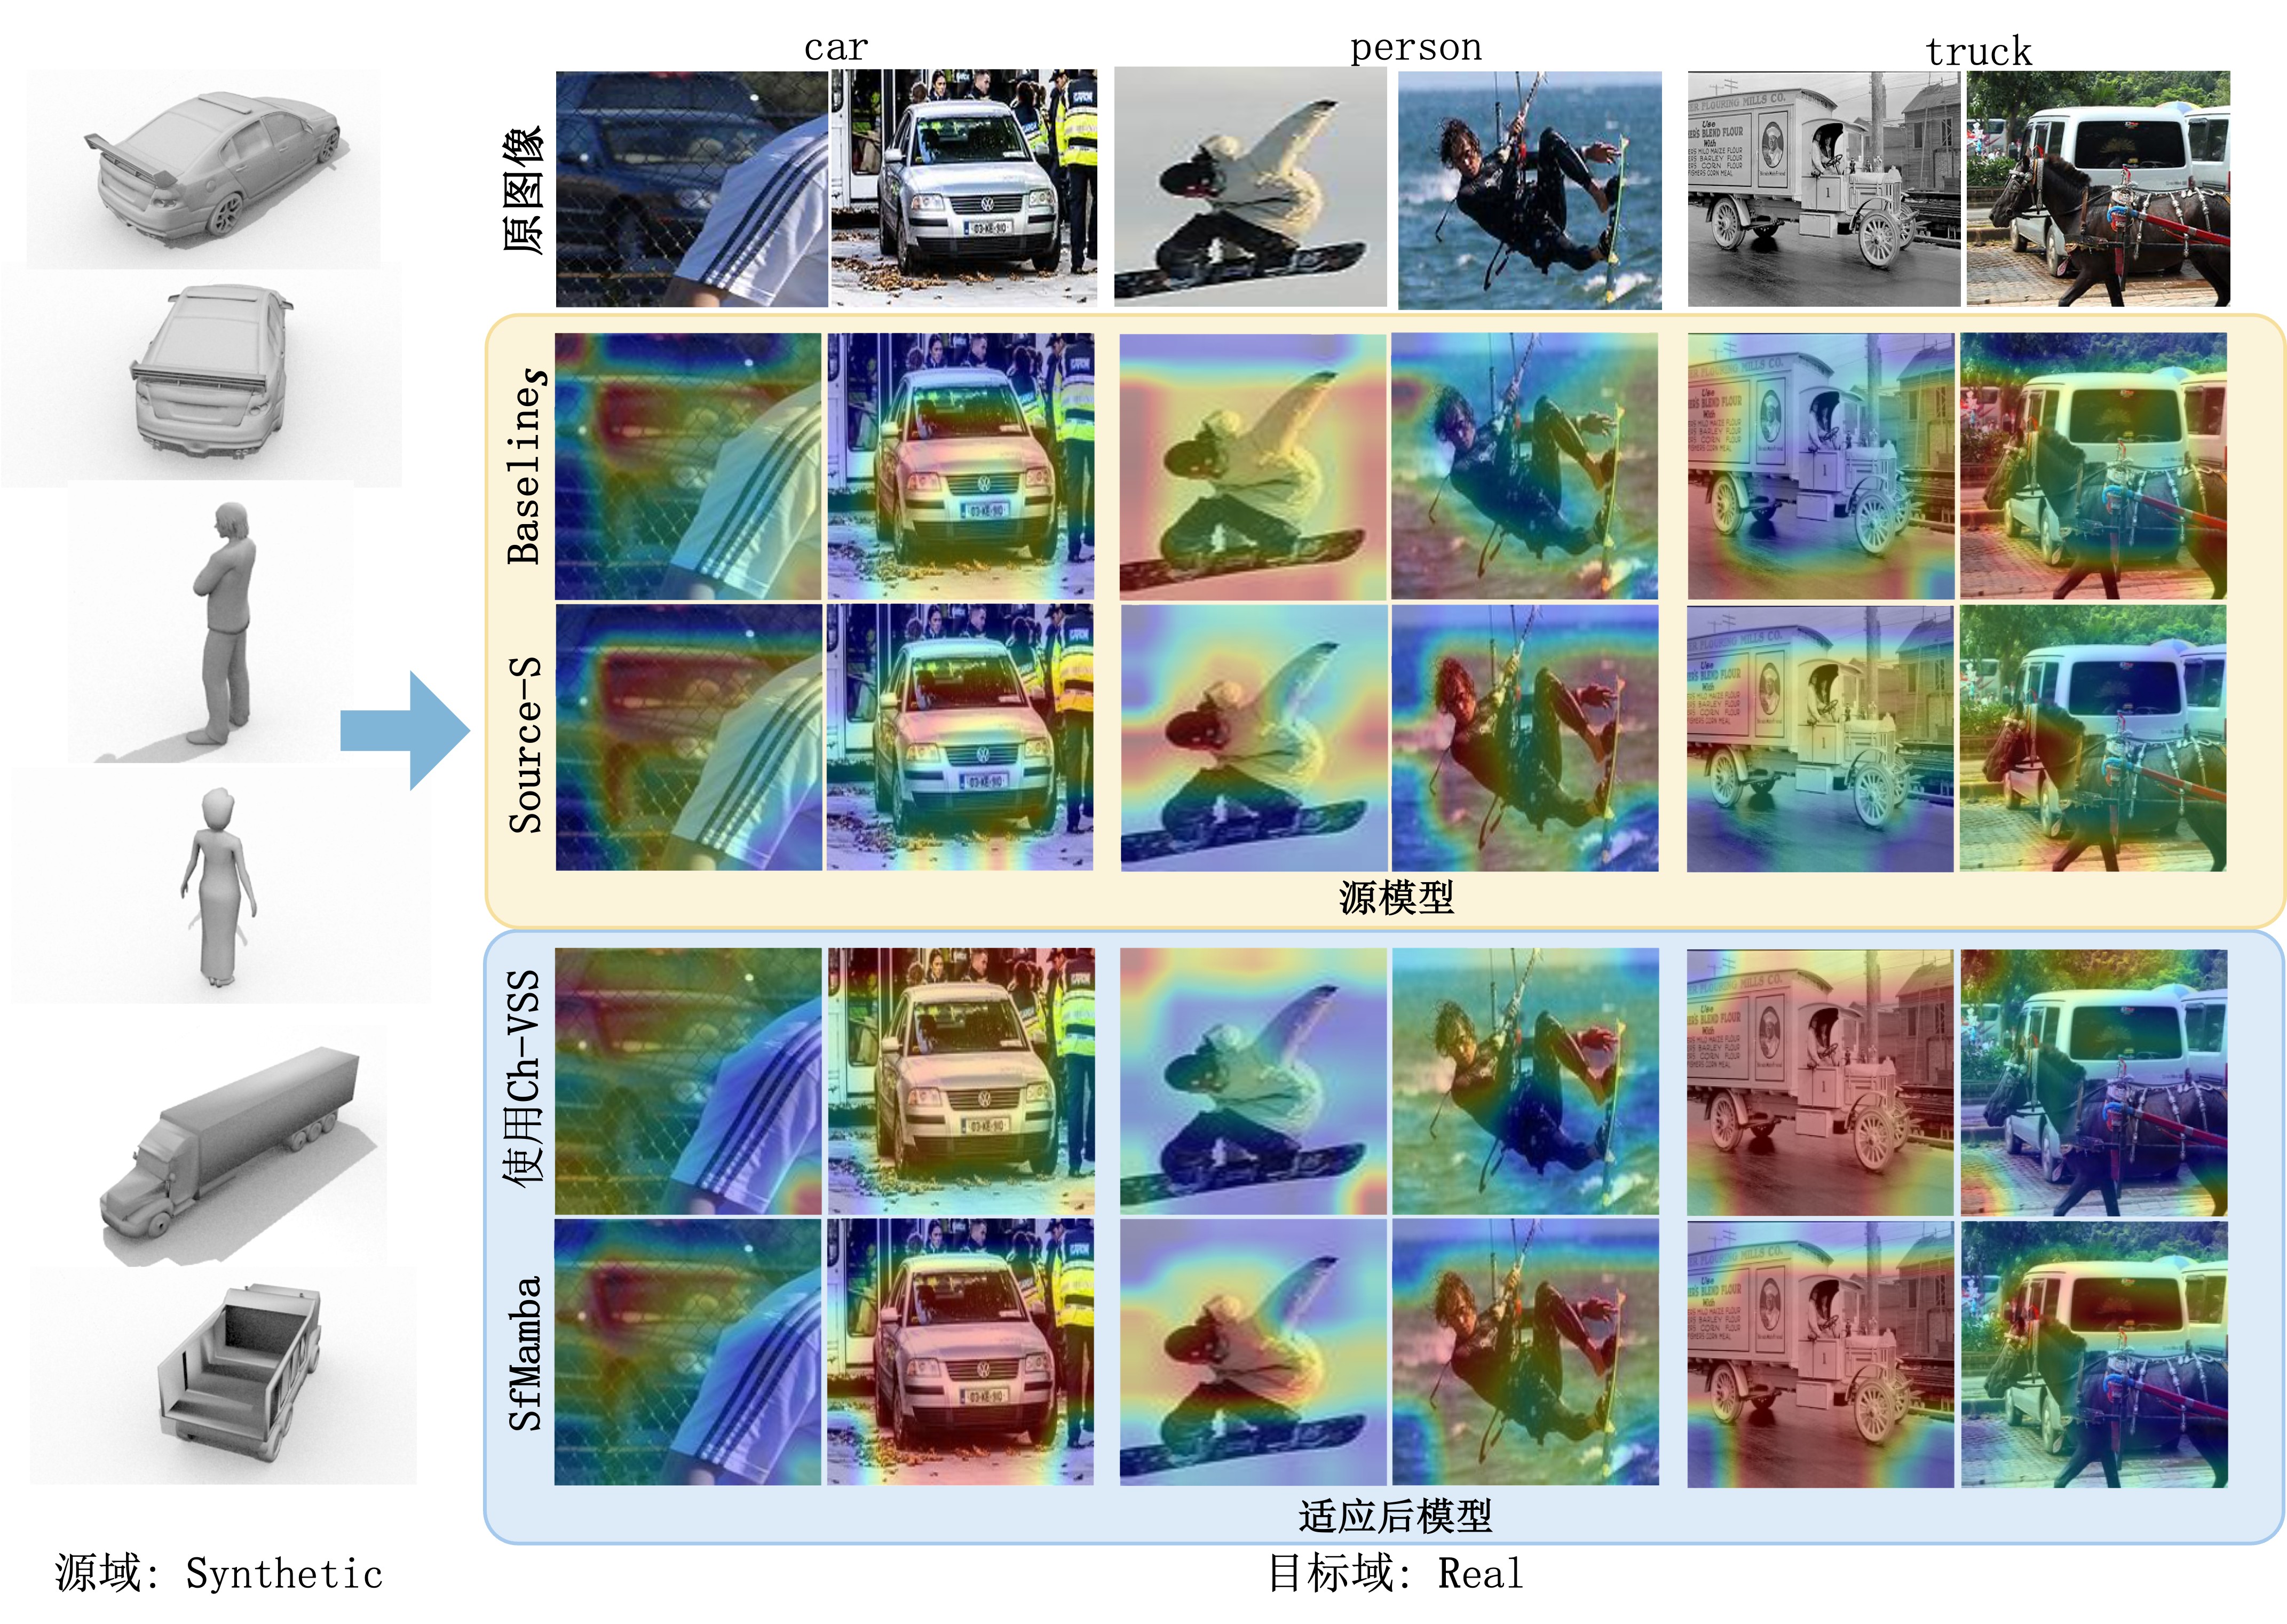
\includegraphics[width=0.9\linewidth]{figures/sfmamba/abl_cam.png}
    \bicaption[fig:sfmamba_gradcam]{}{SCS 模块在 Real 域上的 GradCAM 可视化对比}{Fig.}{GradCAM visualization comparison of the SCS module on the target Real domain of VisDA-C}
\end{figure}

\begin{figure}[!htbp]
    \centering
    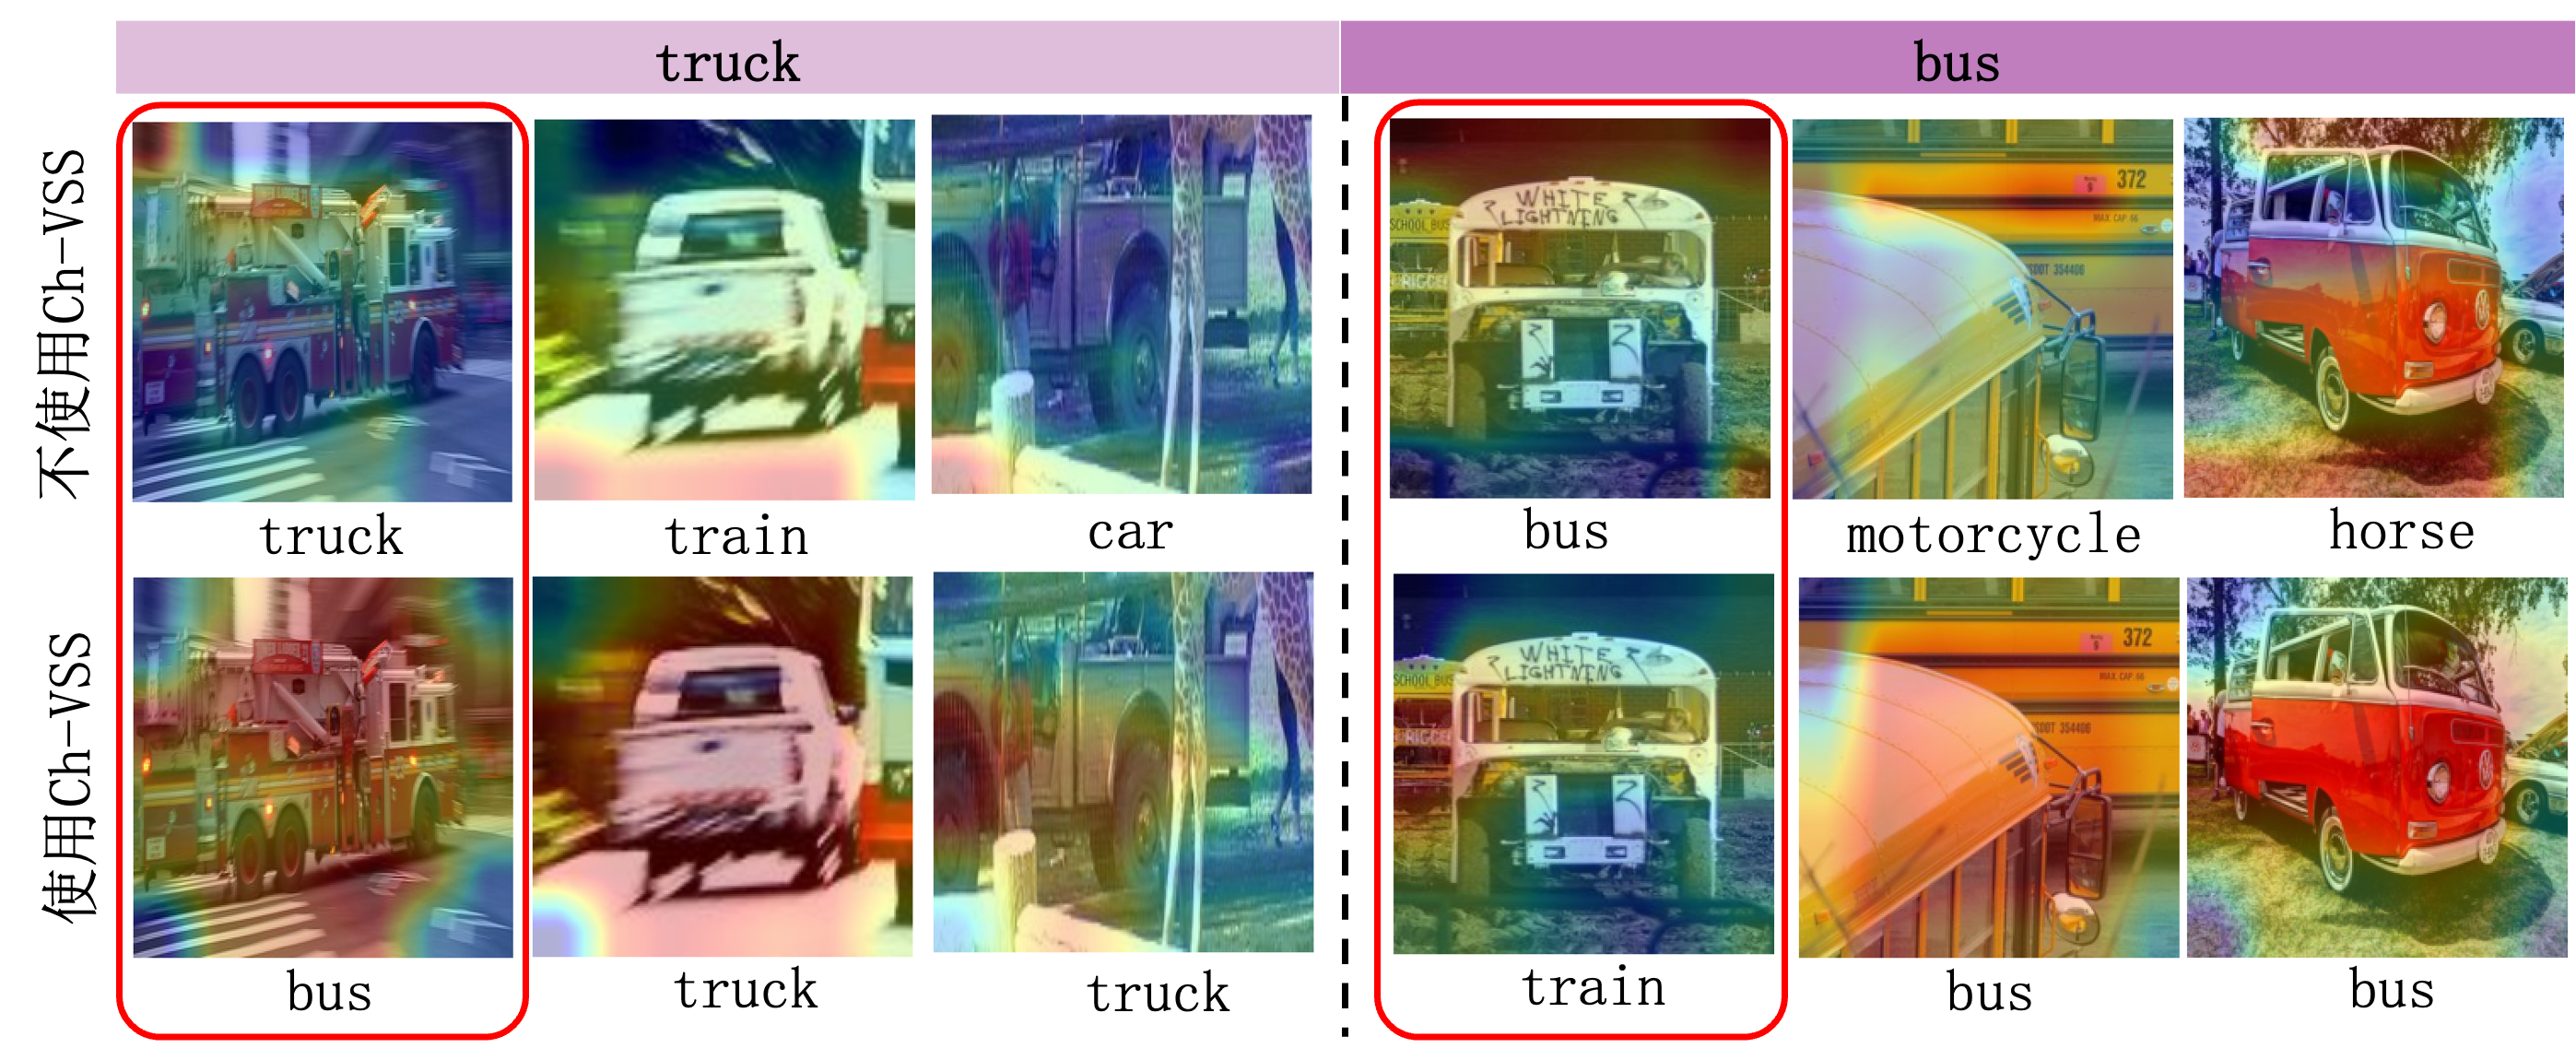
\includegraphics[width=0.8\linewidth]{figures/sfmamba/fail_suc.png}
    \bicaption[fig:sfmamba_cases]{}{SfMamba 在 VisDA-C 上的典型成功与失败案例}{Fig.}{Representative successful and failure classification cases with SfMamba on VisDA-C}
\end{figure}

% \clearpage
\noindent\textbf{（4）超参数分析}

\begin{figure}[!htbp]
  \centering
  \setlength{\tabcolsep}{0pt}
  \subfigure[A$\xrightarrow{}$C]{%
    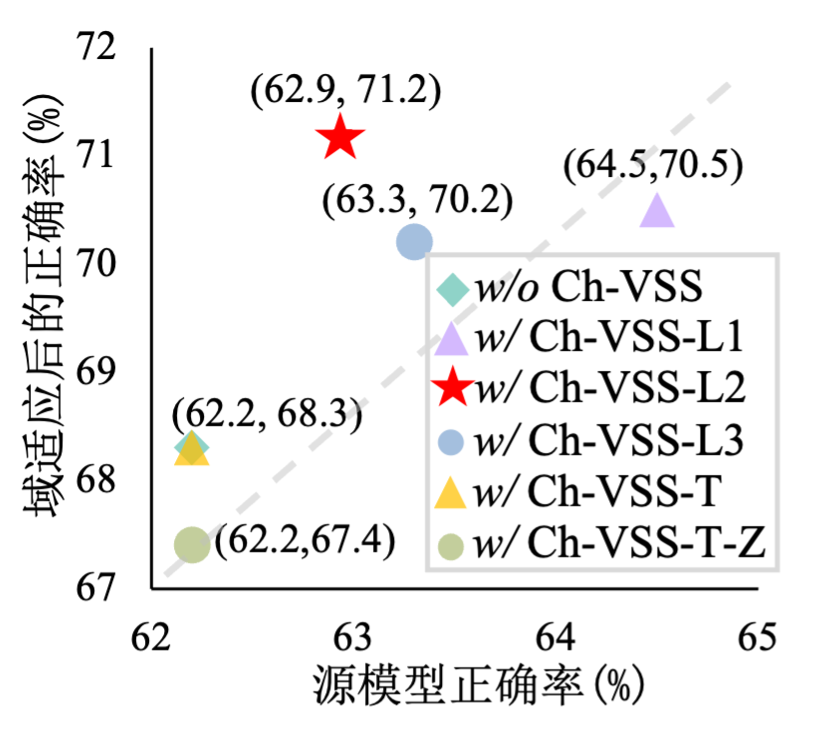
\includegraphics[width=0.48\linewidth]{figures/sfmamba/abl_ch_VSSM_layer_3.png}
    \label{fig:sfmamba_l_ablation_left}%
  }\hfill
  \subfigure[]{%
    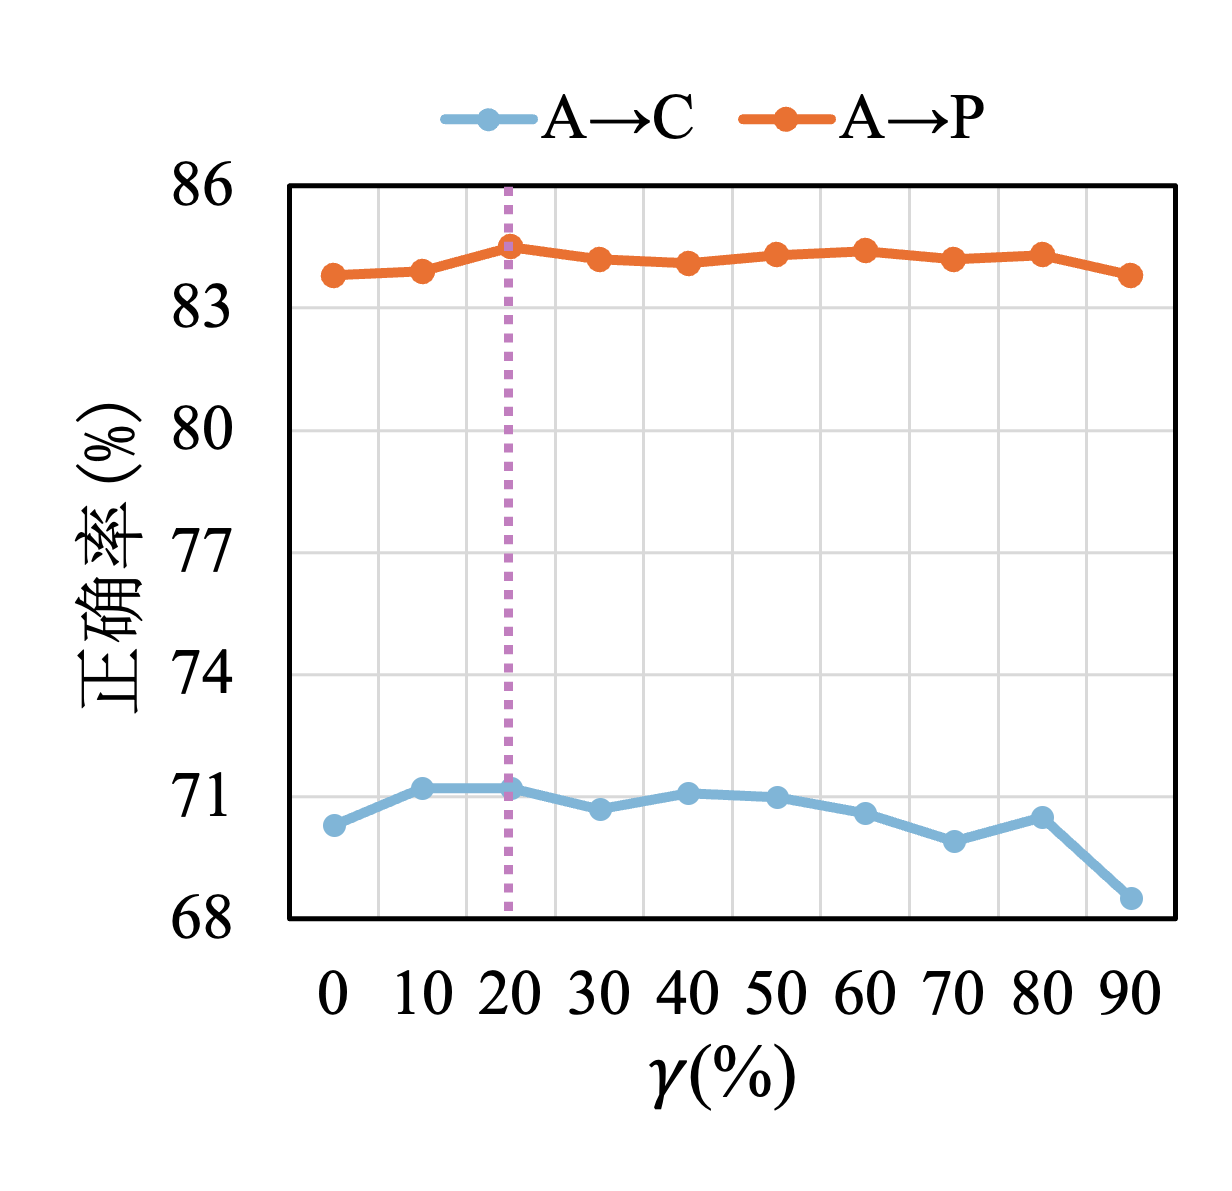
\includegraphics[width=0.48\linewidth]{figures/sfmamba/con_ratio.png}
    \label{fig:sfmamba_l_ablation_right}%
  }
  \bicaption[fig:sfmamba_l_ablation]{}{Ch-VSS 模块数 $L_{\text{vss}}$ 与背景打乱比例 $\gamma_{\text{bg}}$ 的消融}{Fig.}{Ablation on the number of Ch-VSS blocks $L_{\text{vss}}$ and the background shuffle ratio $\gamma_{\text{bg}}$}
\end{figure}

本节考察两个关键超参数：Ch-VSS 块数 $L_{\text{vss}}$ 与 SCS 的背景 patch 比例 $\gamma_{\text{bg}}$。我们记 Ch-VSS 块配置为 Ch-VSS-L$n$，其中 $n$ 表示块数。图~\ref{fig:sfmamba_l_ablation_left} 报告了源域与适应后目标模型在 Office-Home A$\rightarrow$C 任务上的精度。结果显示，引入 Ch-VSS 块始终能提升目标域精度，且 Ch-VSS-L2 配置在目标域上取得最优性能。图~\ref{fig:sfmamba_l_ablation_right} 进一步展示了背景比例 $\gamma_{\text{bg}}$ 对目标精度的影响：当 $\gamma_{\text{bg}}=20$ 时取得最高精度，性能在小 $\gamma_{\text{bg}}$ 值下保持稳定，但 $\gamma_{\text{bg}}$ 过大时显著下降——这与过度打乱会破坏结构化图像内容的预期一致。



\noindent\textbf{(5)计算效率}

图~\ref{fig:acc_pam} 与表~\ref{tab:efficiency} 联合呈现了 SfMamba 在精度—参数量权衡上的优势。VMamba-S 变体以 58.9M 参数、9.2G FLOPs 取得 Office-Home 81.7\%，超越 DeiT-B 基的 CDTrans/DeSiT（80.5\%，86.6M）；VMamba-T 以 39.0M 参数取得 79.2\%，超越同规模 ViT 与 CNN 基线方法。

与 ResNet-101 基的 I-SFDA 相比，VMamba-T 实现减少 4M 参数与 2.4G FLOPs；与 DeiT-B 基的 CDTrans 相比，VMamba-S 减少 32.0\% 参数（27.7M）、47.7\% FLOPs（8.4G），并提升 25.9\% 吞吐量；与 Mamba 基 DATMamba 相比，参数量与 FLOPs 分别减少 38.7M（39.7\%）与 5.8G（38.7\%）。这些结果进一步印证了 SfMamba 在精度—效率双重权衡上的竞争力。

\begin{figure}[!htbp]
  \centering
  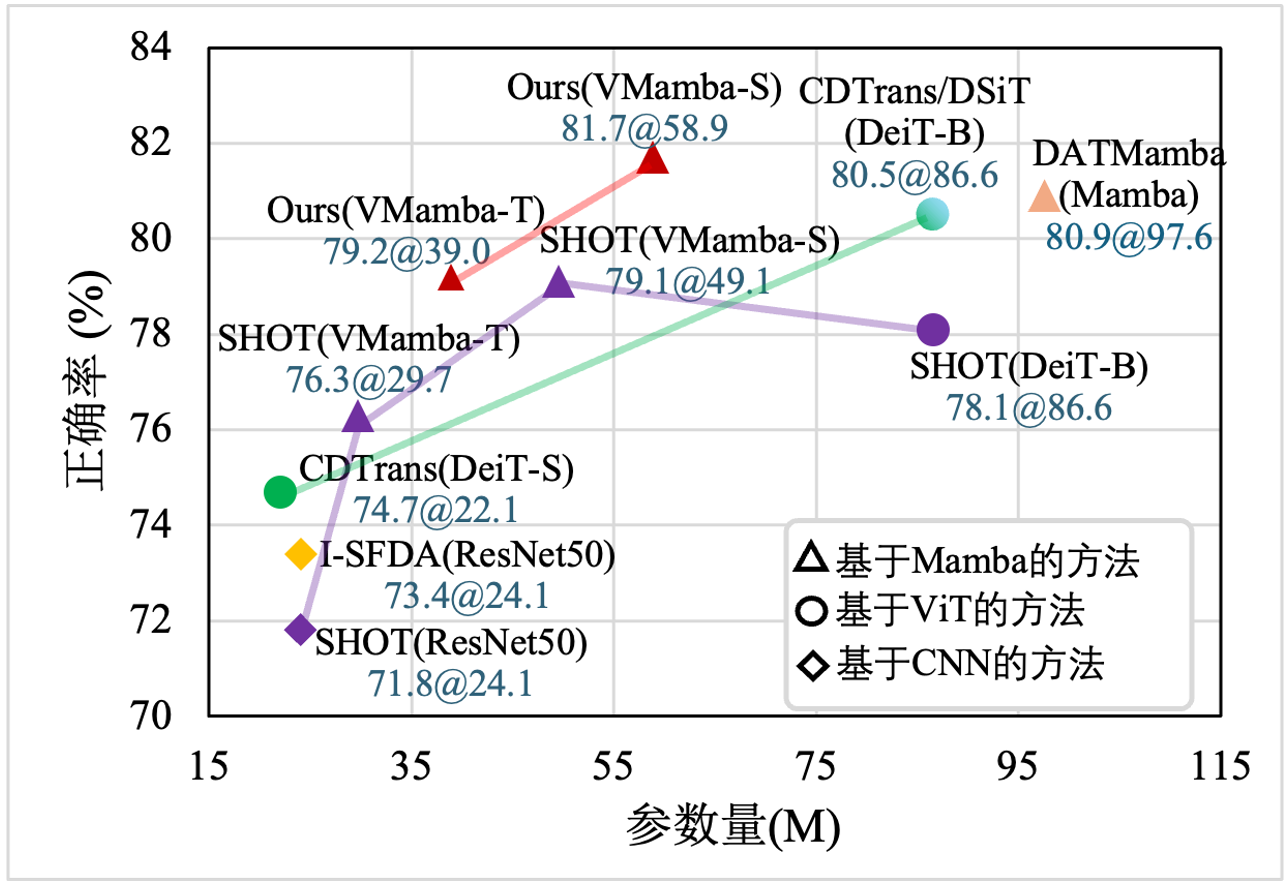
\includegraphics[width=0.7\textwidth]{figures/sfmamba/acc_param.png}
  \bicaption[fig:acc_pam]{}{不同骨干网络在 Office-Home 上的精度—参数量权衡}{Fig.}{Accuracy vs.\ parameter efficiency across backbones on Office-Home.}
\end{figure}
\begin{table}[!htbp]
    \bicaption[tab:efficiency]{}{UPA 与 SfMamba 在计算效率与精度上的综合对比}{Table}{Computational efficiency comparison}
    \vspace{0.5em}\centering\wuhao
    \resizebox{\textwidth}{!}{
    \begin{tabular}{llcccc}
    \toprule
    方法 & 骨干网络 & 参数量 (M) $\downarrow$ & FLOPs (G) $\downarrow$ & 吞吐 (img/s) $\uparrow$ & Office-Home (\%) / VisDA-C (\%) \\
    \midrule
    % UPA & ResNet-50/101 & 23.5 / 42.5 & 4.1 / 7.8 & -- & 73.0 / 88.7 \\
    I-SFDA~\cite{mitsuzumi2024understanding} & ResNet-101 & 43.0 & 7.8 & 1094.7 & -- / 88.4 \\
    SfMamba-T & VMamba-T & 39.0 & 5.4 & 700.9 & 79.2 / 88.5 \\
    \midrule
    CDTrans~\cite{xu2022cdtrans} & DeiT-B & 86.6 & 17.6 & 399.5 & 80.5 / 88.4 \\
    DATMamba~\cite{gao2025datmamba} & Mamba & 97.6 & 15.0 & -- & 80.9 / 88.9 \\
    \textbf{SfMamba-S} & VMamba-S & \textbf{58.9} & \textbf{9.2} & 502.8 & \textbf{81.7 / 89.3} \\
    \bottomrule
    \end{tabular}}
\end{table}




% \textbf{适用场景} 当部署资源严格受限或类别空间较小时，UPA 路线（CNN 骨干 + 伪标签去噪）具有更高的工程性价比；当数据集包含跨域长程依赖或类别空间显著差异时，SfMamba 路线（SSM 骨干 + 通道/空间双向增强）具备更强的精度优势。两条路径在“抑制迁移不确定性”的统一主题下为不同部署需求提供了互补方案。
\FloatBarrier
\section{本章小结}

本章面向无源域适应中源域数据不可访问、目标域无标注所导致的迁移不确定性问题，在统一的伪标签自训练框架下，按不确定性的作用层次展开研究：在判别层，提出基于特征空间邻居结构与类感知对比学习的伪标签去噪方法，从源头抑制噪声在自训练回路中的反复累积，避免引入额外模型；在表征层与序列层，针对状态空间骨干特有的通道建模缺失与空间共现虚假相关，分别以通道维度频率域依赖建模与背景 patch 扰乱稳定跨域表征，以线性复杂度实现高效长程建模。判别层去噪机制在卷积骨干与状态空间骨干上分别得到验证，两个层次在状态空间骨干上叠加使用并取得协同增益。在四个跨域基准上的实验验证了上述不确定性分层抑制机制的有效性。上述结果说明，可靠的目标域监督信号与鲁棒的特征提取机制缺一不可，二者共同构成无源域适应中抑制迁移不确定性的基础。

% Local Variables:% Local Variables:
% TeX-master: "../thesis"
% TeX-engine: xetex
% End:
